\section{Úvod}
\label{sec:Uvod}

V dnešní době automatizace a~digitalizace je třeba využít tohoto trendu a~převést do praxe metody pro zefektivnění práce v těch oblastech, kde to ještě před pár lety kvůli technickým bariérám nebylo možné. Jednou z oblastí, kterou lze moderními technologiemi zefektivnit je urgentní příjem nemocnic. Na toto oddělení, kde hrají i sekundy otázku života a~smrti, je kladen vysoký nárok na monitorování a~sledování ošetřovacího cyklu pacienta. Přínos digitalizace lokace a~provedených ošetřovatelských výkonů v~reálném čase je nezměrný. Například zpětným statistickým vyhodnocením lze posoudit, jaké fáze vyšetření bývají časově nejnáročnější. Vymezením kritických oblastí a~jejich náprav lze zvrátit pomyslný jazýček vah na kladnou stranu při záchraně člověka. Jestliže jsou k~dispozici data v~reálném čase, nic nebrání tomu je logicky a~přehledně zobrazit. Dalším přínosem je tedy nepochybně lepší orientace v~současné situaci pro nově příchozí personál nebo při hromadných nehodách.

Cílem diplomové práce je vytvořit aplikaci pro personál urgentního příjmu Fakultní nemocnice Ostrava, pomocí které bude možné ovládat systém lokalizace v reálném čase (Real Time Location System dále jen RTLS) na uživatelské úrovni. Cílem je tedy v~první řadě seznámit se s~nynější situací na urgentním příjmu, pochopit a~lokalizovat problémy, které trápí toto oddělení. Bylo potřeba se také poučit z~dřívějšího pokusu o~lokalizačním systému pacientů. Poté je cílem tyto poznatky přenést do užitkových a~vývojových diagramů. Na základě těchto komplexních diagramů poté představit návrhy aplikace a~paralelně sestavit backendové prostředí pro chod aplikace. Po schválení návrhu už zbývá jen podle něj naprogramovat skutečnou frontendovou část. V~průběhu vývoje je důležité aktivně komunikovat se zaměstnanci urgentního příjmu a~průběžně konzultovat případné nedostatky či zlepšení. Po odladění obou částí aplikace je třeba nasadit celkové řešení na server nemocnice a~provést konečnou fázi testování v~reálném provozu. 

Celá tato diplomová práce se skládá ze čtyř kapitol. Diplomová práce začíná úvodní první kapitolou, která uvádí čtenáře do problematiky. Další kapitola podrobně popisuje technologie pro tvorbu webových aplikací. Popsané technologie byly vybrány na základě implementovaných technologií nebo z~důvodu toho, že byly předchůdci implementovaných technologií a~bylo potřeba vyzdvihnout jejich rozdíly. Další kapitola pak obsahuje vlastní návrh řešení, v~této části práce je popsána analýza současné situace, postup vývoje a~vysvětlení architektury aplikace. Poslední kapitola pak hodnotí celou práci, nastiňuje budoucí motivaci a~uzavírá tuto diplomovou práci.


\section{Technologie pro tvorbu webových aplikací}

V této kapitole budou popsány technologie a~koncepty, které byly použity v~praktické části nebo mají úzkou spojitosti, bylo nutné je popsat pro vytvoření uceleného obrazu. Jsou také popsány přilehlé oblasti jako komunikace, typy dat či zabezpečení, které souvisí s~touto problematikou.

\subsection{Klient-Server}
\label{sec:KlientServer}

Jde o~typ architektury, která odděluje síťově, topograficky a~logicky část klientskou (dále jen klient) a~serverovou (dále jen server). Některá logika či část programového postupu je vykonávána na klientské straně a~ta druhá část na serveru. Klient překládá klientský požadavek tak, aby byl přijatelný serverem a~čeká od něj odpověď, kterou překládá zpět tak, aby byla srozumitelná klientovi. Ten ji pak na obrazovce prezentuje uživateli. Klient je tedy aplikace na koncovém zařízení uživatele, která je nejčastěji reprezentována rozhraním (interfacem). Serverová část je naopak část, která je mimo uživatelské zařízení. Nejčastěji je reprezentována databází držící data, která jsou pak poskytována klientovi nebo naopak klientem posílána data pro ukládání. Na obrázku \ref{fig:ClientServer} je zobrazena architektura typu klient-server.\cite{1}\\
 
\myparagraph{Výhody} 

Největší výhoda této architektury je jasné oddělení aplikační logiky na dvě části. První částí je klientská strana, která je aktivní, posílá a~přijímá žádosti na nebo ze severu a~druhá část je serverová strana, která je pasivní, naslouchá všem požadavkům na síti, které se správně autorizují. Další výhoda je snadná údržba a~rozšiřitelnost. Například je možné nahradit, opravit, modernizovat, přemístit server, aniž by to klienti poznali, nebo tím byli nějak ovlivněni. Další výhodou je bezpečnost. Tím, že jsou všechna data (i citlivá osobní data) bezpečně uložena na serverech, která jsou bezpečnější než většina klientů, je menší pravděpodobnost úspěšného úmyslného útoku či odcizení. Servery jsou také snadněji kontrolovatelné, co se týče přístupu a~jeho sledování. \\
 
\myparagraph{Nevýhody} 

Za nevýhodu se dá považovat nerobustnost\footnote{Robustný -- program naprogramovaný tak, že se pokusí za každou cenu běžet dál.}. Pokud dojde k~výpadku serveru, veškeré žádosti klientů jsou neobslouženy a~vráceny s~chybovým kódem 5xx, což jsou chybové kódy serveru (většinou jde o~503 Služba nedostupná (Service unavailable)). Mezi další nevýhody řadíme přetěžování sítě. Počet požadavků klientů na server může přesáhnout mez, kterou server zvládne obsloužit. Může dojít ke krachu serveru, který vede k~první nevýhodě (viz. výše). \\
 
Výše zmíněné nevýhody jsou již ale překonány. Nerobustnost řešení lze vyřešit například aplikováním serverových nodů s~loadbalancerem. v~případě, že by některý server vypadl, loadbalancer přesměrovává veškeré požadavky na zbývající žijící nody. Tím je zajištěna robustnost řešení. Další překonanou nevýhodou, která byla popsána výše je přetěžování sítě. Toto lze obejít různými hardwarovými i~softwarovými řešeními, čehož lze dosáhnout limitací požadavků v~časovém intervalu.\cite{2, 3}

\begin{figure}[H]
	\centering
	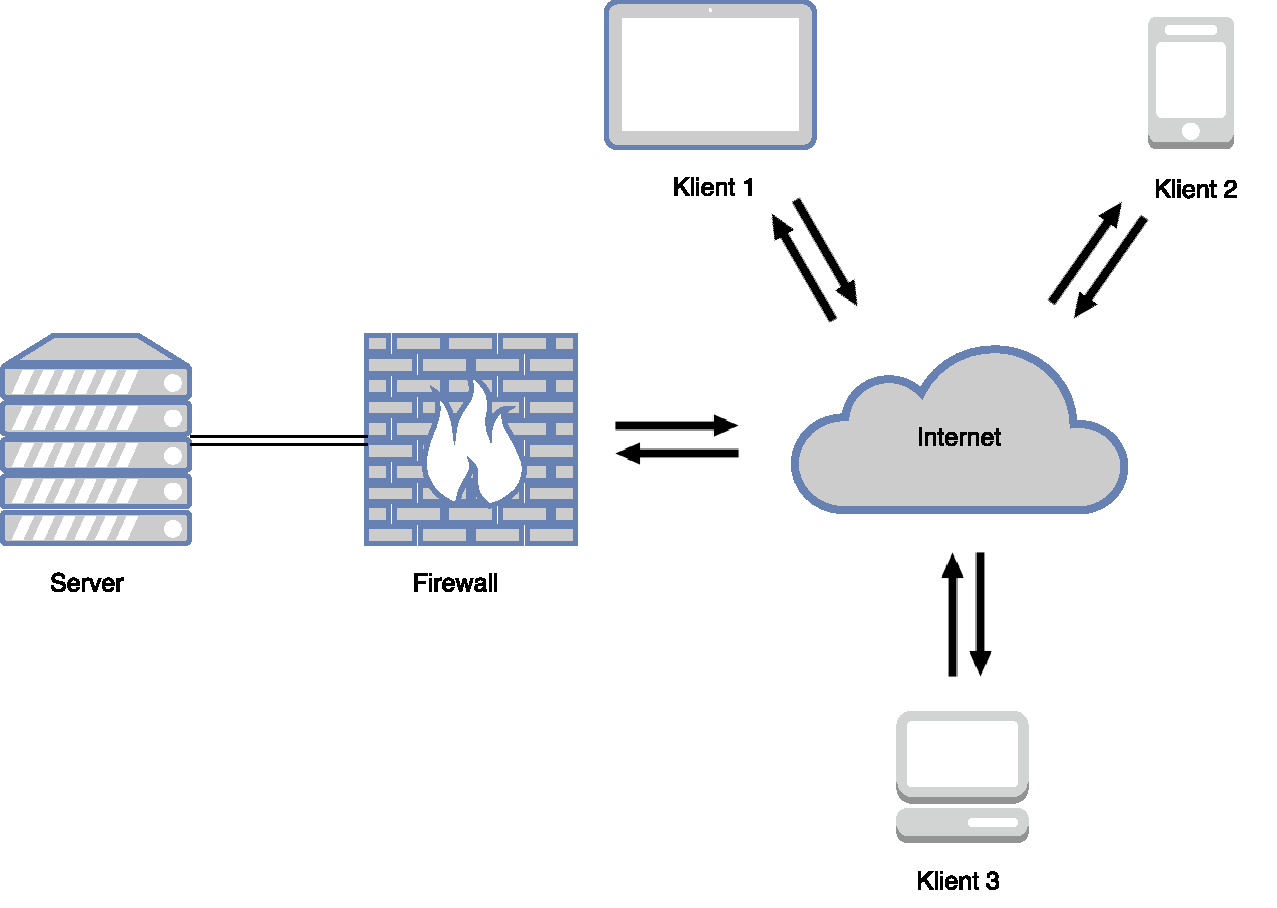
\includegraphics[width=15cm]{../ClientServer.pdf}
	\caption{Topologie sítě klient-server. Na levé straně je serverové prostředí, které může obsahovat více serverů nebo další technologie jako load-balancer, Domain Name Server (dále jen DNS) server, oddělené databázové stroje apod. Serverové prostředí je odděleno firewallem (s nebo bez různých restrikcí) pro bezpečnost před útoky. Příchozí požadavky ze sítě přicházejí přes internet od různých klientů. Klientem může být cokoliv, co dokáže vytvořit a~odeslat správně požadavek. Ten je pak obsloužen serverem a~vrácen zpět. }
	\label{fig:ClientServer}
\end{figure}

\subsubsection{Způsob komunikace}
\label{sec:zpusobKomunikace}

\myparagraph{Hypertextový komunikační protokol}

Hypertext Transfer Protocol (dále jen HTTP) je komunikační protokol, který patří k~nejpoužívanějším způsobům komunikace dvou zařízení. Tento typ funguje způsobem request-response (požadavek-odpověď). Klient pošle serveru dotaz obsahující hlavičku a~tělo dotazu. Hlavička obsahuje různé informace. Například označení požadovaného dokumentu, údaje o~prohlížeči apod. Server přijme (pokud je validní) požadavek a~poté odpoví pomocí několika řádků textu popisujících výsledek dotazu (zda se dokument podařilo najít, jakého typu dokument je atd.), za kterými následují data (pokud byla požadována).
 
Tato komunikace se odehrává po síti, nejčastěji po internetu. HTTP protokol je ovšem nezašifrovaný, nezabezpečený a~nezabezpečující integritu dat kanálu, který lze odposlouchávat, číst cizí informace zvenčí či podsouvat falešná nebo škodlivá data. Tento protokol obvykle používá TCP/80 port. Jak již bylo řečeno, HTTP komunikace je otevřená a~přenášené informace mohou být po cestě mezi klientem a~serverem odposlouchávány. Kdokoliv tedy může číst data, hesla a~další citlivé údaje. Aby se tomuto odposlechu zamezilo, byl vyvinut protokol HTTPS (secured – zabezpečený).\cite{4}
 
Základem zabezpečené komunikace je SSL certifikát, který zajišťuje šifrovanou komunikaci mezi serverem a~klientem. Tento certifikát se skládá z~veřejného klíče a~privátního klíče. Zákaznický certifikát, který je vystavován certifikační autoritou (CA -- certificate authority), je nainstalován na serveru a~tím se také server prokazuje klientovi. Zprostředkující certifikát je oproti tomu nainstalován v~prohlížeči a~během komunikace se jím prokazuje důvěryhodnost certifikátu protistrany. Tento zabezpečený kanál většinou komunikuje na portu TCP/443.\cite{5}

Na obrázku \ref{fig:HTTPS} je popsaný sekvenční diagram procesu HTTPS komunikace. Při první fázi je použit veřejný klíč pro vytvoření zašifrované komunikace. Tato fáze je pouze inicializační a~probíhá jen jednou. Druhá fáze je pak použita při každé další komunikaci a~je použit privátní klíč. 

\begin{figure}[H]
	\centering
	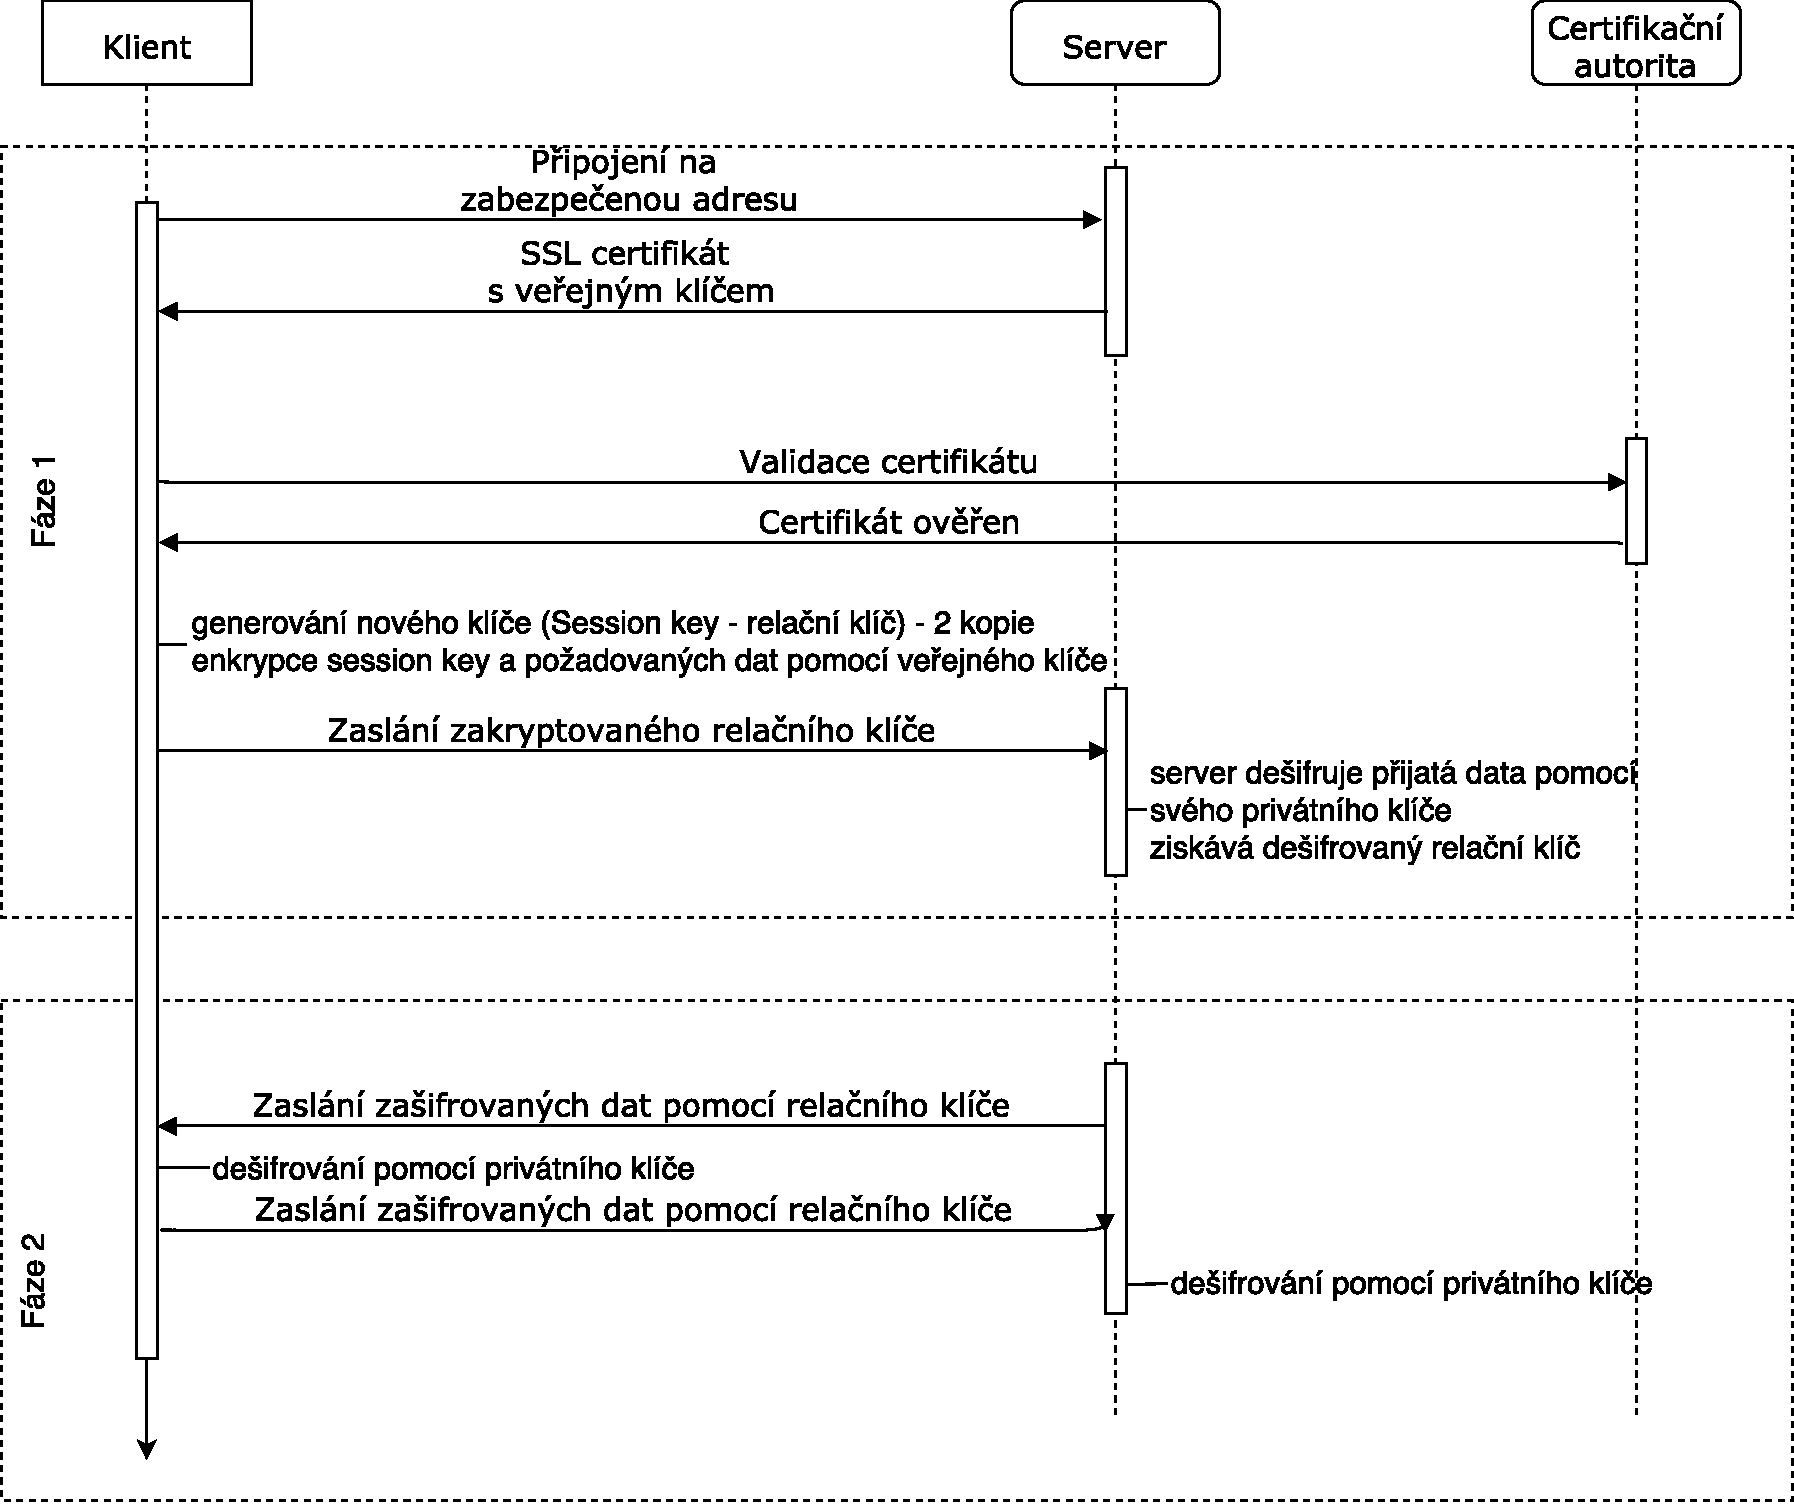
\includegraphics[width=16cm]{../HTTPS.pdf}
	\caption{Aktivitní diagram komunikace HTTPS. v~první fázi je vyslán požadavek klienta na připojení zabezpečené stránky. Server poté vrací certifikát s~veřejným klíčem, který je zpracován po odeslání certifikační autoritou. Klient poté přijímá odpověď (ta je kladná či zamítavá). Klient pak na základě veřejného klíče generuje dvě kopie relačního klíče. Tento klíč s~daty (pokud jsou) je poté pomocí ověřeného veřejného klíče zakryptován a~odeslán na server. Ten následně dešifruje požadovaná data pomocí svého privátního klíče. V~případě úspěchu získává dešifrovaný relační klíč. Tímto krokem končí první fáze, kdy se navzájem ověřují certifikáty. V~druhé fázi už probíhá ověřená komunikace. Po klientském požadavku server odesílá zpět požadovaná data zašifrovaná pomocí relačního klíče. Klient tato data dešifruje s~privátním klíčem a~získává tak dešifrované údaje. V~opačném směru funguje tato fáze stejně. Klient zakryptuje data pomocí relačního klíče a~server poté dešifruje data pomocí svého privátního klíče.}
	\label{fig:HTTPS}
\end{figure}

\myparagraph{RSA šifrování}

Tento typ šifrování se nejčastěji používá pro kryptování privátního klíče. Patří mezi asymetrické kryptografie, přičemž se od symetrické liší tím, že nemá pouze jeden klíč, pomocí kterého se přenášená zpráva šifruje a~inverzním postupem dešifruje. Asymetrické šifry mají klíče dva. Soukromý a~veřejný. Zašifrovaná zpráva je poslána přes nezabezpečenou síť. Obsah zůstane ale utajen v situaci, kdy útočník nemá privátní klíč pro rozšifrování. 
Principem RSA šifrování je předpoklad, že rozložení velkého čísla na součin prvočísel je takřka nemožné. V~procesu faktorizace (rozložení čísla na součin prvočísel), tedy $ n = p.q $, není znám žádný algoritmus faktorizace, který by pracoval v~polynomiálním čase\footnote{Nicméně je očekáváno, že s~příchodem opravdu výkonných kvantových počítačů je tento typ šifrování ohrožen.}.\cite{6}


\subsubsection{Formáty dat}
Pro správný chod aplikací je nutné, aby mezi sebou nějakým způsobem komunikovali přes jakýkoliv komunikační standart (POP3, SMTP, IMAP, HTTP atd.). Existuje mnoho typů dat, ale v~této práci si uvedeme dva nejmodernější a~nejpoužívanější způsoby, jak formátovat data. \\

\myparagraph{Rozšířující značkovací jazyk} \\
Extensible Markup Language (dále jen XML) je značkující jazyk, za jehož vznik a~standardizaci vděčí konsorciu W3C\footnote{World Wide Web Consorcium je mezinárodní společnost, která vyvíjí webové standardy pro World Wide Web.}, slouží pro serializaci dat. Jedná se o~formát dokumentů, který předepisuje, jak zapisovat data společně s~užitečnými daty. XML tagy nejsou předdefinované, lze si tedy definovat své vlastní. Tento jazyk a~jeho kód ve své podstatě nic nevykonává. Pouze drží informaci, kterou přenáší. S~XML lze vyměňovat data i~mezi dvěma naprosto nesourodými systémy.

Tagy je možné předdefinovat v~souboru dokument pro definici typů (Document Type Definition dále jen DTD), jestliže potřebujeme validovat na vstupu xml dokument s~daty ve správném formátu. Lze automaticky kontrolovat, zda vytvářený či přijímaný dokument odpovídá definici, která je v~DTD. Tento validační dokument ale není jediným způsobem, jak zkontrolovat správnost struktury XML dokumentu. Jelikož DTD neobsahuje možnost kontrolovat typy dat (čísla, řetězce znaků apod.), mnohem častěji se používají XML schémata nebo také definice XML schémy (XML Schema Definition (XSD)). 

Další vlastností XML je, že v~jednom dokumentu můžeme používat najednou nezávisle na sobě několik druhů tagů pomocí jmenných prostorů (namespaces). Z~toho plyne, že v~jednom XML dokumentu můžeme používat několik různých DTD nebo schémat bez konfliktů v~pojmenování tagů.\cite{7, 8}

Kódování XML dokumentu je vždy Unicode\footnote{Mezinárodní standard pro kódování znaků.}, kódování lze ale podle potřeb změnit. Aby byl XML dokument považován za správný musí splňovat alespoň následující body:

\begin{enumerate}
	\item Elementy mohou být vnořeny, nemohou se ale překrývat. Znamená to, že každý tag musí být celý v~jiném tagu. Ve výpisu \ref{lst:rootXML} jsou v~našem případě v~tagu \textit{produkt} vnořené tagy \textit{nazev} a~\textit{cena}. 
	
	\pagebreak
	
	\begin{lstlisting}[numbers=none, caption=Ukázka kořenového elementu XML dokumentu., label=lst:rootXML]
	<cenik>
	<produkt kategorie="polevky">
	<nazev>Bramborova polevka</nazev>
	<cena mena="CZK">25</cena>
	</produkt>
	</cenik>
	\end{lstlisting}
	
	\item Jména tagů v~XML rozlišují malá a~velká písmena, tzn. jsou case sensitive. XML tagy ve výpisu \ref{lst:smallAndCapitalLetterXML} jsou od sebe různé a~nelze je proto mezi sebou zaměňovat. \\
	
	\begin{lstlisting}[numbers=none, caption=Malá písmena a~velká písmena v~XML, label=lst:smallAndCapitalLetterXML]
	<food>
	</food>		
	
	<Food>
	</Food>		
	\end{lstlisting}
	
	\item 
	Parametr XML tagu se vepisuje do počátečního tagu, následuje rovnítko a~poté je hodnota parametru ohraničena uvozovkami viz. výpis \ref{lst:parameterXMLs}. \\
	
	\begin{lstlisting}[numbers=none, caption=Parametr XML tagu, label=lst:parameterXMLs]
	<day format="dd.mm.yyyy">20.02.2000</day>
	\end{lstlisting}
	
	Má pouze jeden kořenový (root) element. Vy výpisu \ref{lst:rootXML} je v~našem případě root element \textit{<cenik>}.\cite{9} \\
\end{enumerate}




\myparagraph{JavaScriptová objektová notace}

Dalším druhem zápisu dat je formát JavaScript Object Notation (dále jen JSON). Byl navržen Douglasem Crockfordem a~jeho specifikaci můžeme najít v~RFC 4627\footnote{https://www.ietf.org/rfc/rfc4627.txt}. V~dnešní době patří mezi nejoblíbenější formáty na internetu. JSON vznikl v~dobách, kdy se používal pro výměnu dat převážně formát XML. Tento způsob je opět nezávislý na platformě, která má za funkci ukládání a~výměnu dat mezi různými systémy. I~když tento formát obsahuje v~názvu JavaScript, je tento textový způsob zápisu zcela obecný a~lze použít v~jakémkoliv programovacím nebo skriptovacím jazyce. JSON je jednoduše upravovatelný i~čitelný pro člověka a~je jednoduchý způsob pro uložení a~analýzu dat. 
 
Hlavní charakteristikou JSONu je kolekce párů vlastnost a~jeho hodnota. Základní datové struktury jsou realizovány následovně:
 
\begin{itemize}
	\item \textbf{Objekt} \\
	Tento datový typ je v~JSON formátu znázorněn způsobem neuspořádané množiny párů vlastnosti (property) a~jeho hodnot (value).  Objekt začíná levou složenou závorkou a~ukončen je pravou složenou závorkou. Každá property je oddělena od své hodnoty dvojtečkou a~jednotlivý pár property / value je oddělen čárkou. Na obrázku \ref{fig:JSONObject} je graficky znázorněna stavba syntaxe objektu v~JSONu.
	
	\begin{figure}[H]
		\centering
		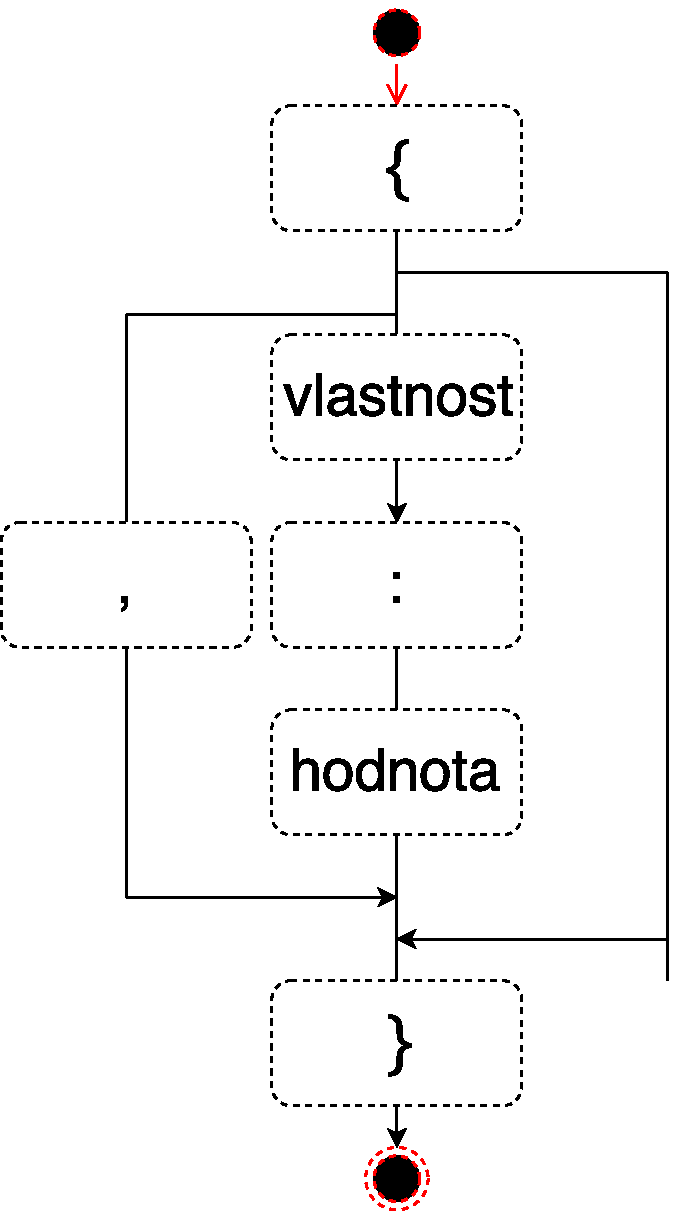
\includegraphics[width=5cm]{../JSONObject.pdf}
		\caption{Zápis objektu v~JSON formátu. Každý objekt začíná levou složenou závorkou. Poté následuje vlastnost oddělená od její hodnoty dvojtečkou. Každý další pár vlastnost-hodnota je poté oddělena čárkou. Výsledný objekt je poté uzavřen pravou složenou závorkou.}
		\label{fig:JSONObject}
	\end{figure}

	\item \textbf{Pole} \\
	Pole je seřazenou kolekcí hodnot. Začíná znakem \textit{[} (levá hranatá závorka) a končí znakem \textit{]} (pravá hranatá závorka). Hodnoty jsou odděleny znakem\textit{,} (čárka). Na obrázku \ref{fig:JSONArray} je graficky znázorněna stavba syntaxe pole v~JSONu.
	
	\begin{figure}[H]
		\centering
		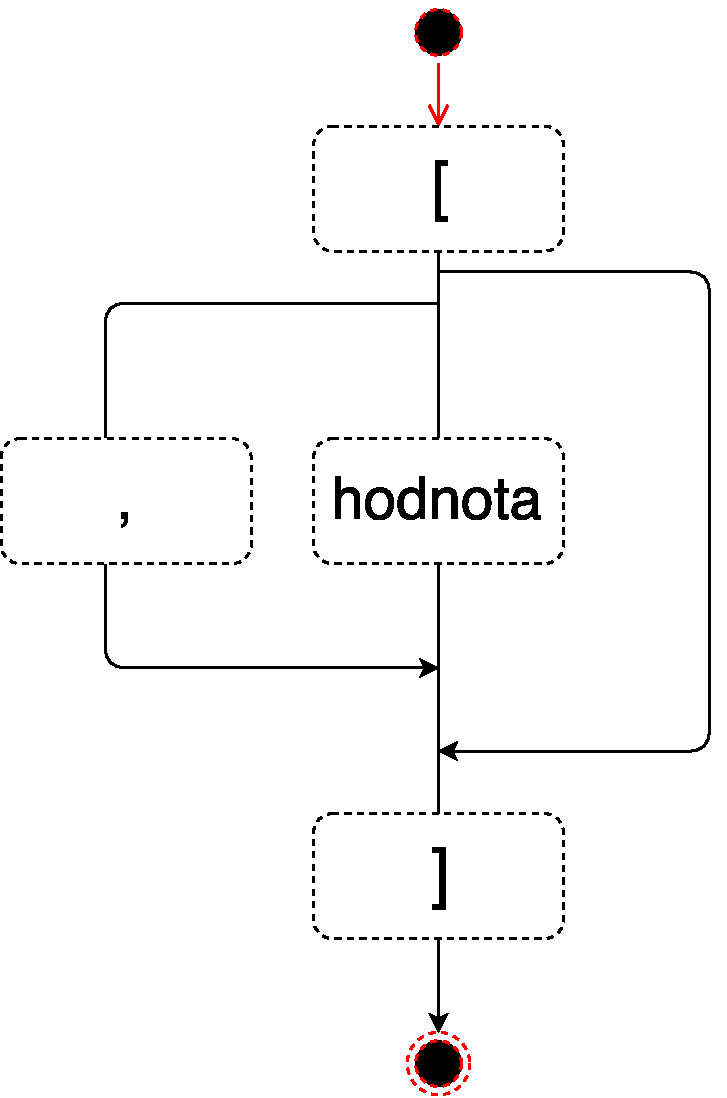
\includegraphics[width=5cm]{../JSONArray.pdf}
		\caption{Zápis pole v~JSON formátu. Každé JSON pole je ohraničené hranatými závorkami. Pole může obsahovat nula a~víc hodnot, které jsou odděleny navzájem čárkou. }
		\label{fig:JSONArray}
	\end{figure}
\end{itemize}

Výhoda JSONu oproti XML je ve velikosti přenášeného souboru. Jelikož je potřeba u~XML otevírací a~zároveň zavírací tag, s~délkou a~komplexnosti struktury dat se zvyšuje i~velikost. Také knihovny pro parsování dat fungují rychleji s~formátem JSON kvůli jednodušší syntaxi. Syntax JSONu totiž mnohem věrohodněji kopíruje objektový svět programovacích jazyků. 
Komplexnost XML přináší ale několik výhod. Mezi výhody patří schopnost lépe zpracovat například fotografie, grafy, zakódovanou hudbu, tedy zkrátka vše, co není primitivní datový typ.\cite{10}

\subsection{Webové technologie}

Tyto aplikace jsou poskytovány uživatelům z~webového serveru poskytovatele přes počítačovou síť internet nebo intranet. Tyto webové aplikace, jak název napovídá, fungují na jakémkoliv webovém prohlížeči, který je v~dnešní době součástí takřka každého operačního systému. Tyto aplikace není nutné nějak instalovat na počítače uživatelů, aktualizovat či mazat. Tyto aplikace běží na standartním formátu HTML/XHTML, který je podporován na všech prohlížečích. Výhodou těchto aplikací je multiplatformnost a~univerzálnost. Místo toho, aby byly psány programy zvlášť pro Windows, Linux nebo Mac OS X, je aplikace napsána v~jednom provedení a~je nabízena komukoliv, kdo přistoupí správně na webový server. Níže si popíšeme vybrané technologie pro tvorbu front–endových částí webové aplikace.

\subsubsection{HTML – Hypertext Markup Language}
\label{sec:HTML}

HTML jazyk je standartní programovací jazyk pro tvorbu World Wide Web (WWW) stránek. Popisuje a~definuje obsah webových stránek nebo aplikace. Dokument v~jazyku HTML má přesně nadefinovanou strukturu a~stejně jako u~XML musí obsahovat kořenový element, hlavičku elementu a~tělo samotného dokumentu. Opět je zde výhoda multiplatformnosti a~univerzálnosti (Vykreslování závisí na prohlížeči a~ne na operačním systému). Společně s~Cascading Style Sheets (CSS), který definuje vzhled a~prezentaci, a~JavaScriptem, který definuje funkcionalitu a~chování, jsou často používány pro vývoj webových aplikací. HTML používá (stejně jako XML) tagy pro anotaci textu, obrázků a~dalšího obsahu ve webovém prohlížeči. Tagy tohoto jazyka mohou buď být v~páru např. <head> a~</head>, přičemž první tag se nazývá otevírací tag a~druhý tag se nazývá ukončovací, nebo se mohou vyskytovat jednotlivě (\textit{<img>}). Zdrojové kódy HTML jsou uloženy v~souboru s~příponou \textit{.html}. Tento soubor je pak načten webovým prohlížečem a~přeloží (vyrendruje) kód do okna prohlížeče. Na obrázku \ref{fig:HTMLElement} vidíme anatomii HTML elementu.

\begin{figure} [H]
	\centering
	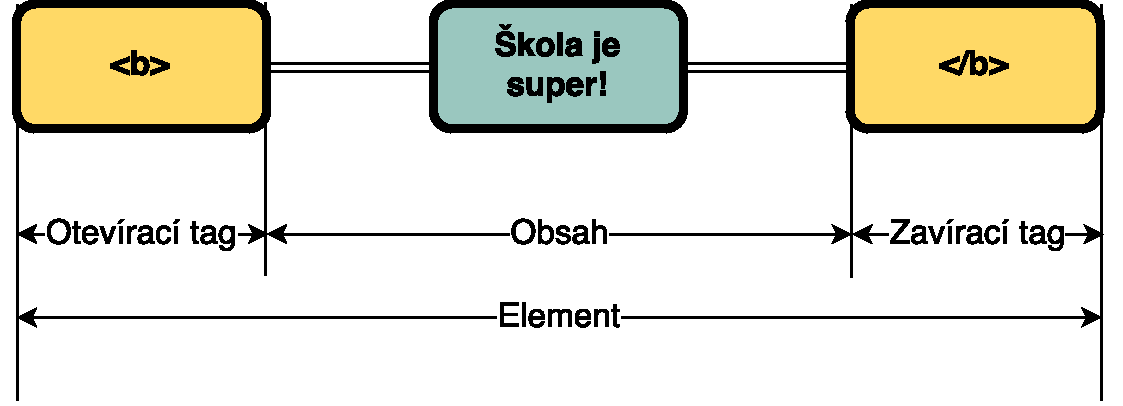
\includegraphics[width=10cm]{../HTMLElement.pdf}
	\caption{Grafické rozložení HTML elementu. Každý HTML tag je uvozen počátečním a~koncovým tagem, přičemý koncový tag obsahuje lomítko před názvem elementu. Mezi HTML tagy je pak daný obsah.}
	\label{fig:HTMLElement}
\end{figure}

Na výpisu \ref{lst:HTML} je znázorněn ukázkový program v~HTML. Vše, co je obsaženo mezi tagem \textit{<body>} a~\textit{</body>}, definuje obsah webové stránky. Zároveň vše, co je mezi tagem \textit{<html>} a~\textit{</html>}, popisuje samotnou webovou stránku. Na příkladu můžeme vidět tag \textit{<p>} a~\textit{</p>} vnořen v~tagu \textit{<body>}. Toto se nazývá vnoření tagů a~vytváří se nám relace rodič-potomek, kde rodič je v~našem případě element \textit{body} a~potomek je element \textit{p}. 
Pro různé přizpůsobení tagů zde existují parametry (atributy) HTML tagu. Tento parametr se zapisuje stejně jako u~XML (viz. výše) např. \textit{<img src='image.jpg'>} nebo \textit{<p align='center'></p>}. Většina parametrů je nepovinná až na ty, které jsou povinné u některých tagů, například \textit{img} má povinný atribut \textit{src} a~\textit{alt} pro správné vykreslení obrázku na stránce.


\begin{lstlisting}[numbers=none, caption=Ukázka HTML dokumentu., label=lst:HTML]
<html>
  <head>
    <title>This is a title</title>
  </head>
  <body>
    <p>Hello world!</p>
  </body>
</html>
\end{lstlisting}



HTML vznikl v~90. letech minulého století a~od té doby se v~programovacím světě změnilo spoustu věcí. Nyní je používaná verze HTML 5, která vznikla v~roce 2014. V~dnešní době se všechny prvky, které jsou v~interakci s~uživatelem přesouvají do CSS jazyka. Přístup komunity programátorů se mění a~cílem je vyvíjet lehce spravovatelné programy a oddělit od sebe funkcionalitou jednotlivé jazyky. Vizuální formatování s~HTML tagy je již tedy zastaralé a~nemělo by se používat. Představme si, že budeme muset změnit font celé webové stránky či aplikace. Pokud bychom postupovali s~klasickým HTML, bylo by nutné přidat, změnit či odebrat hodnotu parametru na každém místě, kde se nachází font. S~CSS jazykem toho jde dosáhnout jednoduše jednou změnou.\cite{11}\cite{12}

\subsubsection{CSS}
\label{sec:CSS}
CSS je jazyk, který, jak již bylo nastíněno výše, popisuje vzhled HTML, XHTML nebo XML a~je nadstavbou těchto dokumentů. V~dnešní době by se už mělo stylovat zásadně pomocí tohoto jazyka a~ne~v~HTML. Hlavní úlohou CSS je tedy oddělení vzhledu od logického obsahu. S~CSS styly lze přiřadit každému tagu v~HTML určité vlastnosti (umístění, způsob zobrazení, vzhled atd.), a~to dokonce i~v~závislosti na jakém rozlišení je HTML dokument vykreslován (obrazovka PC, tiskárna, mobilní telefon, zvukový výstup atd.). V~CSS lze definovat i~pravidla stylů. Styl definuje pravidla, jak prvek různě interpretovat. Takových pravidel může být spoustu. Nejvíce používané jsou např. barva, font, pozice, aj. Kaskádovost stylů je dána hierarchickým uspořádáním pravidel pro styly.

Způsob vytváření stylů je definován seznamem položek. Jednotlivou položkou může být pravidlo ve tvaru \textit{selektor definice}. Selektor určuje, na který prvek se daný styl (pravidla) aplikuje. Definice pravidla, které popisuje konkrétní vlastnosti zvoleného selektoru, má tvar \textit{vlastnost:hodnota vlastnosti}. Každé pravidlo je odděleno středníkem.\cite{11}\cite{12} \\

Příklad definice stylu:
\begin{lstlisting}[numbers=none]
.registratePatientBorder {
    border-width: 0px 1px 0px 0px;
    border-style: solid;
    border-color: black;
    padding: 15px 15px 15px 15px;
}
\end{lstlisting}

Jelikož lze vkládat styly několika~způsoby, tak se určování toho, který styl bude mít nejvyšší prioritu a~použije se pro zobrazení elementu, řídí následujícími pravidly (číslování 1 je s~nejvyšší prioritou a~číslování 3 je s~prioritou nejnižší):

\pagebreak

\begin{enumerate}
	\item Inline styly v~HTML tagu
	\item Externí a~interní styly
	\item Styly definované v~prohlížeči jako základní
\end{enumerate}

\myparagraph{Implementace CSS do HTML}

Jak již bylo řečeno výše, existují tři způsoby, jak vložit styly do HTML dokumentu. Tak, že je definován přímo v~HTML tagu nebo pomocí externího souboru. Tyto metody lze libovolně kombinovat mezi sebou podle účelu. 

Importování externího souboru lze docílit způsobem, že mezi HTML tagy \textit{<head>} a~\textit{</head>} vepíšeme tag \textit{<link>} či \textit{<style>} přes který se importuje námi zvolený externí css soubor. \\ 

\begin{center}
	\textbf{Příklad: } <link rel="stylesheet\textquotedbl \ type="text/css" \ href="app.css" /> 
\end{center}
 
Inline styl lze implementovat pomocí tagu <style> přímo uvnitř dokumentu. Tohoto způsobu využijeme pokud máme jednotný styl a~vzhled celé webové aplikace a~chceme u~jedné části použít jiné pravidlo.

\begin{center}
	\textbf{Příklad: }  <p style="color: green\textquotedbl>Tento obor je super!</p> 
\end{center}

Importování interního vloženého stylu se docílí způsobem, že je daný selektor ohraničen \textit{<style>} tagem.

\myparagraph{Příklad: }  
\begin{lstlisting}[numbers=none]
<style>
	p {
		color: green;
	}
</style> 
\end{lstlisting}

Když webový prohlížeč zobrazuje dokument, musí v~první řadě skombinovat obsah samotného dokumentu a~jeho styly. Tento krok probíhá ve dvou fázích:

\begin{enumerate}
	\item Konverze HTML a~CSS do Document Object Model (dále jen DOM).
	\item DOM je pak uložen v~paměti operačního systému. 
	\item Prohlížeč následně zobrazí obsah DOMu.
\end{enumerate}

Na obrázku \ref{fig:CSSLoad} je znázorněno načtení HTML dokumentu s~CSS styly.

\begin{figure} [H]
	\centering
	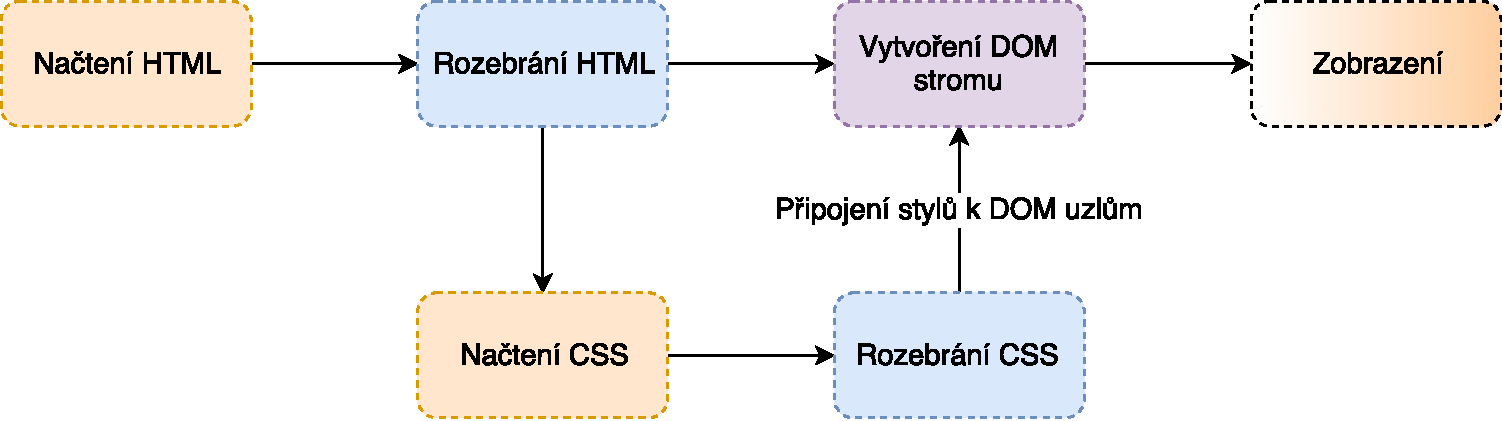
\includegraphics[width=14cm]{../CSSLoad.pdf}
	\caption{Načtení HTML a~CSS prohlížečem. Po načtení HTML je prohlížečem tento dokument rozebrán přičemž zjistí lokaci CSS souborů. Styly jsou poté rozebrány a~společně s~HTML je vytvořen DOM, který je pak uložen v~paměti operačního systému. Prohlížeč poté zobrazí obsah DOMu.}
	\label{fig:CSSLoad}
\end{figure}

\subsubsection{JavaScript}
\label{sec:JavaScript}
Javascript je multiplatformní, skriptovací a~objektově orientovaný jazyk. Tento jazyk stejně jako HTML (kapitola \ref{sec:HTML}) a~CSS (kapitola \ref{sec:CSS}) bývá implementovaný na straně klienta (ačkoliv open sourcový projekt Node.Js je JavaScriptový framework pro práci na straně serveru) např. webový prohlížeč. Byl vyvinut v~roce 1995 Brendanem Eichem\footnote{Programátor původem z~USA, který vytvořil skriptovací jazyk Mocha. Poté byl přejmenován na LiveScript a~ve stejný měsíc byl finálně změněn na JavaScript.} ze společnosti Netscape, který byl jako poprvé nasazen ve stejnojmenném prohlížeči. Tento skriptovací jazyk pak byl následně implementován i~v jiných prohlížečích konkurenčních firem. v~roce 1997 byl jazyk standardizován a~byla vytvořena specifikace ECMA-262, která byla podporována ve všech známých prohlížečích. Od té doby vzniklo 8 verzí ECMA scriptu (k roku 2017) díky kterému je JavaScript jeden z~nejpoužívanějších jazyků v~současnosti. Jelikož jde o~interpretovaný (skriptovací) jazyk tak má oproti kompilovanému mnoho nevýhod a~byl spousta vývojáři a~komunitami odsouzený jako jen jednoduchý nástroj pro oživení stránek. Tento předsudek je ale snad v~této době již překonán. Úspěch jazyka je zejména v~jeho jednoduchosti použití. Na obrázku \ref{fig:htmlCssJs} je znázorněna struktura webové stránky, která implementuje všechny tři technologie. JavaScript tedy umožňuje vytvářet dynamické změny obsahu, kontrolování multimédií, animování obrázků a~další akce, které umožňují interagovat s~uživatelem. \\
\begin{figure} [H]
	\centering
	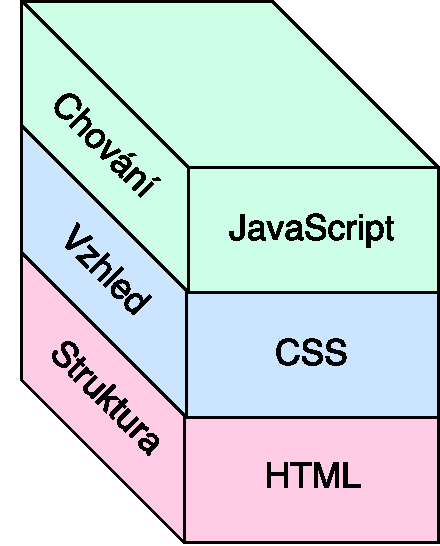
\includegraphics[width=4cm]{../htmlCssJs.pdf}
	\caption{Struktura webové aplikace. Na tomto obrázku je znázorněna stavba a~vrstva jednotlivých technologií. Nejspodnější vrstva HTML zabezpečuje strukturu a~základní kostru webové stránky či aplikace. Následuje soubor stylu, který se stará o~vzhled dané stránky. Nejvýše je položena vrstva s~JavaScriptovým kódem, který má na starosti chování aplikace. Všechny tyto tři vrstvy dohromady dávají stavbu moderní webové stránky.}
	\label{fig:htmlCssJs}
\end{figure}

Syntaxe jazyka se podobá jazyku C, C\# a~Java a~má rysy imperativního, strukturovaného, dynamického, funkcionálního a~v neposlední řadě, jak již bylo řečeno, je to objektově orientovaný jazyk.

\myparagraph{Imperativní a~strukturovaný jazyk}

Imperativní a~strukturované programování je jedno ze základních programovacích paradigmat. Imperativní neboli procedurální programování popisuje úkon nebo výpočet pomocí posloupnosti příkazů a~určuje přesný postup (algoritmus), jak danou úlohu řešit. v~reálném světě je tohle například kuchařský recept či návod k~sestavení nábytku z~IKEY. Strukturované programování je další paradigma, které je založené na cyklech a~větvení programu. Problém se rozloží na několik podproblémů a~každý podproblém potom řeší určitá funkce s~parametry. \\

\myparagraph{Dynamický jazyk}

Jazyky, které jsou dynamické fungují tak, že za běhu provádí většinu činnosti, kterou by kompilované jazyky již dělaly během doby kompilace. Datové typy jsou dynamicky určovány za běhu programu. Lze taky měnit objekty i~celého objektového modelu za běhu a~funkce eval umožňuje vykonávat nový kód v~JavaScriptu předaný této funkci jako řetězec. \\

\myparagraph{Funkcionální jazyk}

Funkcionální paradigma je založeno na zápisu programu ve tvaru výrazu. Funkce lze předávat jako argument, vracet jako výsledek a~přiřazovat do proměnných. Dalším znakem funkcionálního programování u~JavaScriptu je zanořování funkcí, které umožňují definovat funkce v~rámci jiné funkce. Dále uzávěry (closures) umožňují při invokaci zanořené funkce přístup k~proměnných ze svého oboru platnosti (scope) i~když k~zavolání dojde úplně v~mimo obor platnost (out of scope). \\

\myparagraph{Objektově orientované programování -- OOP}

Toto paradima vychází od imperativního (procedurálního) programování. Tento model se skládá spíše z~objektů než z~akcí a~dat než z~logiky. Kvůli zapouzdření a~abstrakci jsou metody (funkce) zapouzdřeny v~objektech. Nutno podotknout ale, že v~JavaScriptu se objekty nedefinují pomocí tříd (objektů), ale pomocí funkcí. Dědičnost se u~tohoto jazyka realizuje trošku odlišným způsobem než v~klasických kompilovaných jazycích. Dědičnost se obvykle realizuje pomocí vlastnosti \textit{prototype} objektu, ve kterém je odkaz na objekt, pomocí kterého byl objekt vytvořen. Ukázka OOP je uvedena v~příkladu \ref{lst:OOP}.\cite{13}\cite{14}

\begin{lstlisting}[numbers=none, caption=Ukázka OOP v~JavaScriptu, label=lst:OOP]

this.pozdrav = null;

function Zvire() {
  this.ozviSe = function() {
    console.log(this.pozdrav);
  }
}

var zvire = new Zvire();

function Pes() {
  this.pozdrav = "Haf Haf"
}

// nastavime do vlastnosti prototype instanci parent objektu se kterym podedi i~jeho metody
Pes.prototype = new Zvire();

// vytvorime instanci child tridy
var benny = new Pes();

benny.ozviSe(); // v konzoli bude "Haf Haf"
\end{lstlisting}

Při načítání webové stránky do prohlížeče je tedy použit kód (HTML, CSS a~JavaScript) pro mechanismus vykreslení. Poté co je HTML a~CSS sestaven a~zobrazen je JavaScript spuštěn překladačem v~prohlížeči. Tím je zajištěno, že struktura a~styl stránky jsou již zavedeny, než se spustí JavaScript. Toto je chování, které je zamýšleno schválně -- totiž velmi častým používáním jazyka JavaScript jsou dynamické úpravy kódu DOMu (HTML a~CSS) pro aktualizaci uživatelského rozhraní prostřednictvím rozhraní API\footnote{Rozhraní (procedury, funkce, třídy apod.) pro programátory, které může využít.} Document Object Model (jak je uvedeno výše). Pokud by JavaScript byl načten dříve a~pokusil se spustit, došlo by k~chybám.

Je důležité se nějakým způsobem chránit před potenciálním škodlivým kódem. Každé okno prohlížeče má svoje oddělené funkční prostředí (Execution environments) což znamená, že JavaScriptí kód, který běží v~jednom okně nemůže ovlivňovat vedlejší stránku či jeho kód. \\

\myparagraph{Implementace JavaScriptu do HTML}

\begin{enumerate}
	\item Inline JavaScript kód (nedoporučuje se)
	\item Interní JavaScript kód
	\item Externí Javascriptí kód
\end{enumerate}

\myparagraph{Inline JavaScript kód}

Někdy se můžeme setkat s~tímto výskytem JavaScriptu, který se nachází přímo v~HTML tagu. Na~příkladu \ref{lst:inlineJS} lze vidět, že HTML tag \textit{<button>} má parametr \textit{onClick}. Tento handler se spouští když je tlačítko spouštěno a~volá JavaScript funkci nadefinovanou výše. Ačkoliv je tenhle kód plně funkční, neměl by se používat. Tenhle přístup nerespektuje oddělení logických vrstev viz. obrázek \ref{fig:htmlCssJs}. v~tomto příkladu se spojuje vrstva strukturální a~behaviorální. Nedoporučuje se zanášet javascript snippety do HTML a~také je tenhle způsob značně neefektivní. Pro správné chování tlačítka bychom museli definovat parametr \textit{onClick} u~každého tlačítka, který by byl v~HTML dokumentu. \\

\begin{lstlisting}[numbers=none, caption=Ukázka inline JS kódu, label=lst:inlineJS]
<button onClick="handleButtonClick()"></button>
\end{lstlisting}


\myparagraph{Interní JavaScript kód}

Dalším způsobem jakým můžeme použít JavaScript v~HTML dokumentu je vepsáním JavaScriptí části mezi \textit{<script>} a~\textit{</script>} HTML tagy viz. příklad \ref{lst:internalJS}.

\pagebreak

\begin{lstlisting}[numbers=none, caption=Ukázka interního JS kódu, label=lst:internalJS]
<script>
	function handleButtonClick() {
		var p = document.createElement('p');
		p.textContent = 'Klikl jste na tlacitko!';
		document.body.appendChild(p);
	}
	
	var buttons = document.querySelectorAll('button');

	for (var i = 0; i < buttons.length ; i++) {
		buttons[i].addEventListener('click', handleButtonClick);
	}
</script>
\end{lstlisting}

\myparagraph{Externí JavaScript kód}

Posledním a~doporučeným způsobem, jak importovat JS kód je následující příklad \ref{lst:externalJS}. Jako v~případě interního JS kódu používáme tag \textit{<script>} jen s~tím rozdílem, že použijeme atribut \textit{src} kde naimportujeme zvolený JS soubor s~naším kódem. Tímhle máme přehledně oddělené logické části webové aplikace.\cite{15}

\begin{lstlisting}[numbers=none, caption=Ukázka externího JS kódu, label=lst:externalJS]
<head>
	<script src="script.js"></script>
</head>
\end{lstlisting}


\subsubsection{AngularJS}
\label{sec:AngularJS}

Nárůst obliby této technologie a~javascriptu obecně přišel s~nástupem HTML5. Tehdy už přestávala knihovna jQuery stačit z~jednoho fundamentálního důvodu. Spojoval dohromady manipulaci s~DOMem, zpracování události a~aplikační logiku. Jelikož se s~přibývajícím výpočetním výkonem a~optimalizací na straně klienta se více a~více logiky přesouvaly směrem ke klientovi bylo následkem, že se kód rozrůstal a~nabýval na komplexnosti. Je nutné si uvědomit, že tehdy neexistoval klientský jazyk, který by ctil architekturu MVC (viz. kapitola \ref{sec:ReactJS}), a~proto se v~roce 2009 poprvé objevil JavaScript framework AngularJS. Autorem je společnost Google a~je jeden z~klientských javascriptích nástrojů, který je meziplatformním řešením pro vytváření aplikací v~klientských částí webové technologie. Je nutné se uvědomit, že před AngularJS nebyl způsob, jak vytvořit dynamické aplikace, kde se informace ve View neustále mění. AngularJS tedy rozšiřuje dokument HTML o~spousty atributů a~elementů, které v~základu chybí.  s~postupem času se tento framework dynamicky měnil, zlepšoval a~narůstal na oblibě. Mezi jeho přednosti je nutno zmínit Two Way Data Binding, Dependency Injection, Testovatelnost, Directives. Jak již bývá zvykem, žádný framework není dokonalý a~i~tento má svoje mouchy. Paradoxně některé jeho přednosti jsou zároveň jeho největšími slabinami. \\

\myparagraph{Dvoucestná synchronizace dat -- Two Way Data Binding}

Tento koncept řeší synchronizaci stavů mezi modelem a~view. Na obrázku \ref{fig:ngTwoWayDataBinding1} a~\ref{fig:ngTwoWayDataBinding} a~příkladu \ref{lst:ngTwoWayDataBindingSourceCode} je znázorněna jednoduchá aplikace, kde máme textové pole a~pod ním vypisujeme obsah pole s~přidaným textem. Ve chvíli kdy proběhne změna v~textovém poli, se text přenese do modelu a~poté se zapíše do části view. Tato automatizace je obsažena ve fundamentálních základech AngularJS a~není proto potřeba se o~nic starat. 

\begin{figure} [H]
	\centering
	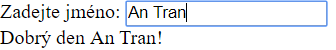
\includegraphics[width=9cm]{../Angular1.png}
	\caption{Ukázka dvoucestné synchronizace dat.}
	\label{fig:ngTwoWayDataBinding1}
\end{figure}

\vspace{5mm}

\begin{lstlisting}[numbers=none, caption=Zdrojový kód ukázky obrázku \ref{fig:ngTwoWayDataBinding}, label=lst:ngTwoWayDataBindingSourceCode]
<div ng-app="MyApp" ng-controller="MyCtrl">
  <p> Zadejte jmeno: <input type="text" ng-model="name"><br>
  Dobry den <span ng-bind="name"></span>!</p>
</div>
\end{lstlisting}

\vspace{5mm}

Ve výpisu \ref{fig:ngTwoWayDataBinding1} vidíme v~HTML tagu \textit {input} přidanou AngularJS direktivu \textit{ng-model}, který přesouvá do jeho modelu (v našem případě \textit{name})  to co jsme napsali do textového pole. Další řádek obsahuje HTML tag \textit{span} s~direktivou \textit{ng-bind}, který má za úkol vypsat všechna data, který obsahuje model \textit{name}. Tímto jsme zajistili deklarativní způsob implementace což znamená funkční automatizovanou dvoucestnou synchronizaci dat. 

\begin{figure}[H]
	\centering
	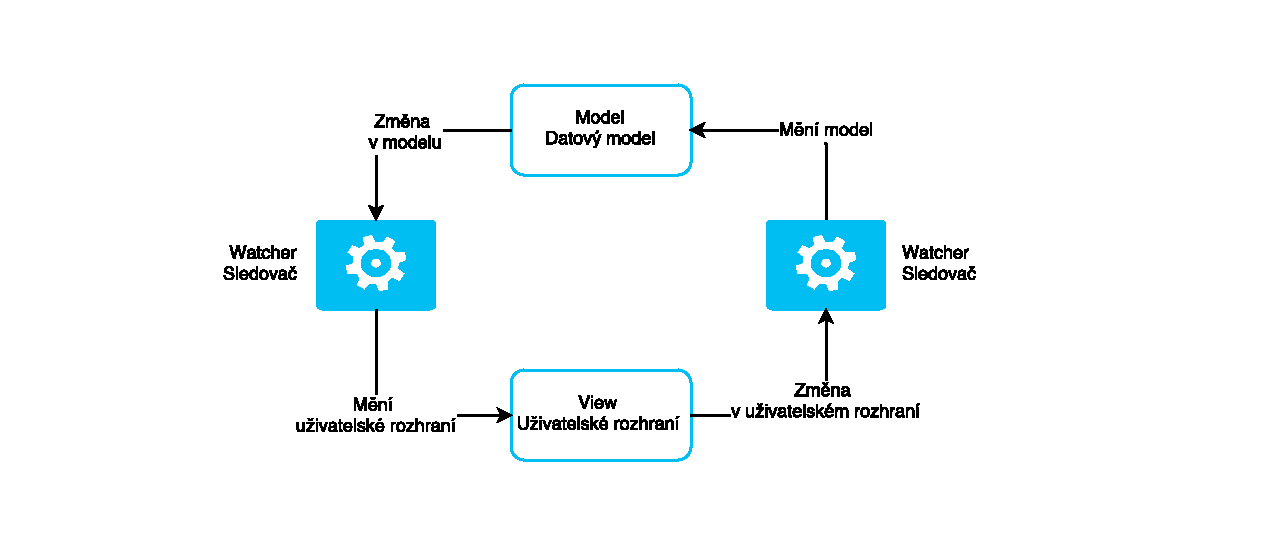
\includegraphics[width=20cm]{../TwoWayDataBinding.pdf}
	\caption{Grafické znázornění dvoucestné synchronizace dat. Zde je graficky znázorněn, jak AngularJS zajišťuje modifikaci datového modelu a~uživatelského rozhraní. Ve chvíli kdy proběhne změna v~textovém poli, se text přenese do modelu a~poté se zapíše do části view. }
	\label{fig:ngTwoWayDataBinding}
\end{figure}

Další výhodou tohoto přístupu je že můžeme model vypsat na více místech view. Změnou dat v~modelu se synchronizuje view na všech místech kde je namapovaný daný model. Tím odpadá povinnost sledovat, kde všude je daný výpis a~synchronizace je spouštěna automaticky.

Jak již bylo řečeno, největší výhody AngularJS jsou zároveň i~jeho nevýhody a~jeden z~důvodů proč byl nahrazen verzi 2.0, který samotnou AngularJS architekturu kompletně obměňuje. Největším problémem je náročnost tohoto přístupu. Na každou direktivu \textit{ng-bind} jsou totiž zaregistrovány sledovače (watcher) a~tedy s~přibývající velikostí aplikace narůstá i~počet watcherů, který sleduje a~naslouchá každé změně. Tím narůstá náročnost aplikace a~klesá její výkon. Dalším důvodem je, že ztrácíme plnou kontrolu nad elementy kdy se mají obnovovat a~také u~větších aplikací ztrácíme přehled odkud byla synchronizace spuštěna pokud potřebujeme zpětně zjišťovat příčinu chyby. Na obrázku \ref{fig:ngTwoWayDataBinding} je znázorněno schéma, jak probíhá dvoucestná synchronizace dat. \\


\myparagraph{Vkládání závislosti -- Dependency Injection}

Dependency Injection (dále DI) je programátorský přístup architektury, který řeší závislost mezi danými komponentami v~aplikaci. Vkládá závislosti mezi komponentami (třídami) bez nutnosti referenci na sebe v~době chodu programu. AngularJS framework obsahuje zabudovaný systém pro DI, který řeší tyto závislosti v~celé aplikaci. v~aplikaci proto pouze specifikujeme, které komponenty jsou používané jinými komponentami. AngularJS dokáže říct, která konkrétní komponenta potřebuje tu danou vyhledáním specifických parametrů konstruktoru\footnote{Metoda, která se zavolá vždy když je vytvářena nová instance komponenty (třídy).}. V~ukázce \ref{lst:ngDependencyInjection} je deklarace kontroleru, kterému se při vytvoření předávají tři parametry, přes které jsou předávány závislosti. Jakmile systém vytváří novou instanci kontroleru, zkontroluje si jeho závislosti v~deklaraci a~všechny předá jako parametry. V~kontroleru se poté pracuje s~závislostmi, které se nazývají služby (services). Interní služby se prefixují znakem dolaru (\$). Ve ukázce \ref{lst:ngDependencyInjection} používáme tři služby: \textit{scope}, \textit{routeParams} a~\textit{location}. \\

\begin{lstlisting}[numbers=none, caption=Ukázka vkládání závislosti, label=lst:ngDependencyInjection]
function ShowInfoPageCtrl($scope, $routeParams, $location) {
  //obsah controlleru
}
\end{lstlisting}

Jelikož vkládání závislosti je zajištěno přes jméno parametru (AngularJS volá interně metodu \textit{toString()}\footnote{Překonvertování daného zdroje na typ string.}, čímž získá jména argumentů, které poté prohledává v~celém listu existujících závislostí), dochází k~problému kdy je zdrojový kód minifikován\footnote{Proces odstranění všech nepotřebných znaků ze zdrojového kódu bez změny jeho funkčnosti.}. Poté co proběhne minifikace, vkládání závislosti přestává fungovat, protože již nenajde zminifikovaný parametr v~seznamu závislostí. Programátoři AngularuJS přišli s~dvěma řešeními pomocí kterých lze tenhle problém obejít. Oba~způsoby jsou naznačený v~ukázkách \ref{lst:ngDependencyInjectionFix1} a~\ref{lst:ngDependencyInjectionFix2}. \\

\begin{lstlisting}[numbers=none, caption=Vložení závislostí v~poli, label=lst:ngDependencyInjectionFix1]
module.controller('ShowInfoPageCtrl', ['$scope', '$routeParams', '$location', ShowInfoPageCtrl]);
\end{lstlisting}

\vspace{5mm}

\begin{lstlisting}[numbers=none, caption=Vložení závislosti do vlasnosti \textit{\$inject}, label=lst:ngDependencyInjectionFix2]
ShowInfoPageCtrl.$inject = ['$scope', '$routeParams', '$location'];
\end{lstlisting}

Tento framework registruje všechny závislosti v~globální hash-mapě což znamená následující nepříjemnost. Pokud je zaregistrována závislost pod stejným jménem dvakrát, novější registrace bez notifikace přepíše tu první. Tento nedostatek vede k~nespočtu chybám v~runtime aplikace a~ke~ztracenému času než je chyba nalezena.  \\

Je nutné podotknout, že AngularJS jako framework byl popisován pro verzi 1.X. Vyšší verze (2.0 a~výš) již tyto problémy překonaly ale došlo k~fundamentálním změnám úplných základů architektury. Vyšší verze je tudíž nekompatibilní s~verzi starší.\cite{16, 17}

\subsubsection{ReactJS}
\label{sec:ReactJS}

ReactJS (nebo také React nebo React.js) je opensourcový\footnote{Projekt, který lidé mohou modifikovat a~sdílet, protože jejich zdrojové kódy js veřejně přístupné.} projekt, který zveřejnil v~roce 2013 Facebook po interním užívání a~odlazování. React přináší zásadní změnu v~paradigmatu, který spojuje dohromady programování a~HTML\footnote{Tato zásadní změna přinesla zezačátku Facebooku ohromnou vlnu kritiky, kdy přemýšlel nad stáhnutím tohoto frameworku.}. v~této práci byl právě použit tento framework jako front-endová část aplikace, proto bude popsána detailněji s~dalšími technologiemi, které se k~Reactu pojí. 

Jak již bylo řečeno, největší výhodou Reactu je, že se tvůrci soustředili na hlavní účel Javascriptích frameworků a~to je View v~MVC architektuře. Tvůrci se poučili s~chyb předešlých frameworků a~cílem bylo vyvinout prostředí, které je lehce udržovatelné, testovatelné a~škálovatelné. React tedy dokáže upravovat DOM pouze deklarativním definováním HTML struktury pomocí JavaScriptích funkcí. Uvedeme tedy, jak má vypadat výsledný View na základě přichozích dat. React framework si poté složí svůj virtuální DOM, který pak optimalizovaně porovnává s~vykresleným DOMem a~vykresluje pouze rozdíly mezi virtuálním a~skutečným DOMem. Tímto výrazně optimalizujeme rychlost klientské části aplikace. \\

\myparagraph{Model View Controller}

Pro kompletní obrázek o~Reactu je potřeba popsat, co to vlastně MVC architektura je.
%https://martinfowler.com/eaaDev/uiArchs.html

\begin{figure}[H]
	\centering
	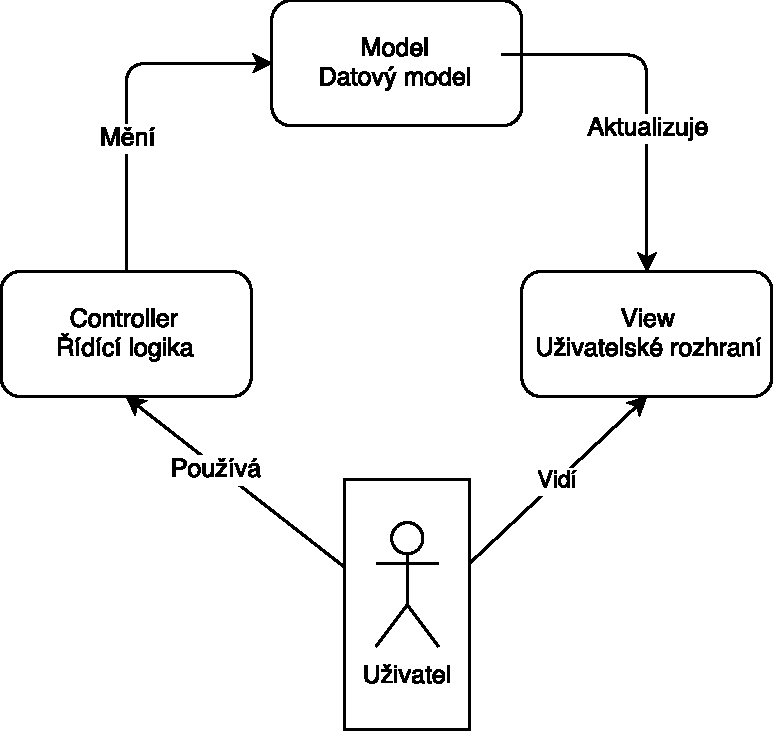
\includegraphics[width=11cm]{../MVC.pdf}
	\caption{MVC architektura.}
	\label{fig:MVC}
\end{figure}

Model-View-Controller (dále jen MVC) je jeden z~nejpoužívanějších a~nejobecnějších architektonických vzorů, který se uchytil zejména na webu, ačkoli původně vznikl na desktopových aplikacích. MVC můžeme rozdělit do tří základních komponent viz. obrázek \ref{fig:MVC}. 

\begin{itemize}  
	\item Model – data a~související operace (tzv. business logika). Model neví, odkud data přišla a~ani, jak budou výstupní data zformátována a~vypsána.
	\item View – prezentace dat (např. uživatelské prostředí) obsahuje přímý odkaz na model, aby mohl jeho data prezentovat vnějšímu světu. View podobně jako Model vůbec neví, odkud mu data přišla, stará se jen o~jejich zobrazení uživateli.
	\item Controller – řadič, který řídí tok událostí v~programu (tzv. aplikační logika) obsahuje přímý odkaz na model, aby mohl modifikovat jeho data.
\end{itemize}

Motivací MVC je oddělení vrstev logiky, dat a~výstupu. Řeší tedy staré programovací neduhy minulého století kdy se v~jednom souboru či třídě střetávaly části, které řeší logické operace (mapování, databázové dotazy, volání cizích systémů či knihoven) a~zároveň vykreslování výstupu. Čili je cílem oddělit tři logické části tak, aby je šlo upravovat samostatně a~dopad změn byl na ostatní části co nejmenší. 

% TODO: REMOVE IF THEY CRY
Popišme si tedy MVC architekturu na něčem co všichni dobře známe a~to stránky s~pornografickým obsahem. \\
View je v~našem případě to co jako uživatel vidíme a~to jest série videí, které si můžeme prohlídnout, reklamy na zázračné prodloužení části těla či náruživé dámy z~okolí. \\
Model jsou data, které jsou uchovávány za vrstvou View. v~našem případě to jsou obrázky, videa, text a~informace o~herečkách atd. \\
Kontroler je nejhůře představitelnou částí na uvedeném příkladu. Projeví se ve chvíli, kdy uživatel interaguje s~dynamickými komponentami ve View. Příkladem je kliknutí na tlačítko přehrát video. Po kliknutí je odstartována kaskáda operací, která má v~tu chvíli na starost, aby se aktualizoval model, došlo k~logickým operacím (kontaktování serveru pro data) a~v poslední řadě překreslení (render) View. Controller je tedy jakousi ústřední výkonnou jednotkou, která se stará o~celkové provázání funkčnosti aplikace.
 
Co je tedy ReactJS v~MVC architektuře? React ve své základní podstatě je pouze View -- uživatelské prostředí. Naším úkolem je tedy pouze dodat nová data do Reactích komponentů a~o zbytek se postará vnitřní algoritmy frameworku. \\

\myparagraph{Komponenty} 

Komponenty (components) jsou základním stavebním kamenem celého ReactJS. Tyto komponenty, které dokážou fungovat samostatně a~jsou navzájem nezávislé, můžeme libovolně kombinovat mezi sebou a~tvořit tak složitější velkopodnikové (enterprise) aplikace. Tato filozofie, která razí stavět složité komponenty z~menších a~znovupoužitelných komponent získala velikou oblibu a~programatorskou základnu tohoto JS frameworku. Všechny komponenty jsou tvořeny popisem, jak by měl View vypadat. Popis je konstruován pomocí JSX (viz. níže) jazyka. Na příkladu \ref{lst:reactComponent} je popsána jednoduchá komponenta, která vykresluje element div obsahující obyčejný textový řetězec. \\

\begin{lstlisting}[numbers=none, caption=Příklad React komponenty, label=lst:reactComponent]
export default class Login extends React.Component {
  render() {
    return(
      <div>Ahoj svete!</div>  
    );
  }
}
\end{lstlisting}

Komponenta má pouze jednu povinnou funkci a~to \textit{render()}. v~ní je popsáno, jak má daná komponenta ve výsledku vypadat v~závislosti na tom jaké data jí budou popsána. Každá metoda \textit{return()} musí vracet jeden kořenový (root)  element (nejčastěji se používá element <div>). Tento kořenový element již může obsahovat nespočet dalších elementů. \\

\myparagraph{Java Serialization to XML (dále jen JSX)} 

V předchozí kapitole Komponenty bylo zmíněno JSX. Zápis JSX je velice podobný HTML (XML) a~jde pouze o~zjednodušení zápisu, který je poté čitelnější a~srozumitelnější. Tento zápis není povinný, nicméně silně se doporučuje při práci s~Reactem. 


na
\begin{lstlisting}[numbers=none, caption=Ukázka JSX a~jeho transkompilaci., label=lst:JSX]
// JSX kod
<CustomJSX irony="true" color="blue">
  Biomedicina je super!
</CustomJSX>

// se kompiluje na
React.createElement(
  CustomJSX,
  {color: 'blue', irony: 'true'},
  'Biomedicina je super!'
)
\end{lstlisting}


Jak vidíme z~příkladu \ref{lst:JSX}, JSX je pouze syntax sugar\footnote{Nahrazení zápisu za jiný o~stejné funkcionalitě za účelem zjednodušení zápisu či zlepšení čitelnosti.}, který se poté kompiluje na funkcí Reactu. První část JSX určuje jméno Reactí komponenty. Velké písmeno názvu označuje, že značka JSX odkazuje na komponentu Reactu. Tyto značky se kompilují do přímého odkazu na danou proměnnou, takže pokud používáte JSX \textit{<CustomJSX />}, \textit{<CustomJSX />} musí být v~rozsahu (scope). \\

\myparagraph{Document Object Model} 

Document Object Model (dále jen DOM) je způsob, jak reprezentovat strukturované dokumenty skrze objekty. Jedná se o~objektově orientovanou reprezentaci HTML nebo XML dokumentu. Také to je API, které umožňuje přístup či modifikaci obsahu. Pokud vztáhneme DOM k~HTML tak HTML je text a~DOM je jeho abstrakce v~paměti prohlížeče. DOM je multiplatformní a~umožňuje prezentaci a~interakci s~daty například v~HTML nezávislou na jazyce. Proto operace, které lze provádět nad DOMem jako hledání uzlů, změna hodnot, odebrání uzlu apod. můžeme docílit pomocí JavaScriptu nebo CSS jelikož samotnou režií operací už má na starosti prohlížeč. Motivací Virtual DOMu (viz. níže) pro vývojáře Reactu je, že DOM nebyl nikdy navržen pro dynamické vykreslování UI\footnote{UI nebo-li User Interface je na první pohled viditelný objekt uživatelem. UI je zjednodušeně řečeno pouze vzhled aplikace.}. \\

\myparagraph{Virtual DOM}

Myšlenka Virtuálního DOMu kterou implementovali vývojáři a~komunita do React frameworku je jedna ze zásadních novinek, která značně optimalizuje celou klientskou část aplikace. Místo přímé interakce s~DOMem, je vytvořena jeho abstraktní (virtuální) verze. Dále pracujeme pouze s~touto odlehčenou abstraktní verzí. Můžeme jej libovolně měnit, přidávat, odebírat atd. a~všechny změny pak najednou uložit do reálného DOMu. Další optimalizací je, že při ukládání do reálného DOMu, ukládáme pouze ty části, které se změnily. Poté pouze tyto změny překreslíme (re-render) a~docílíme toho, že není změněna celá stránka ale pouze ty části, které potřebujeme. \\

Koncept, kterého zanechal tento framework je při každé změně dat přerendrovat celou stránku (nainicializovat všechny komponenty znova, zavěsit listenery atd.). Jelikož jsou komponenty Reactu předpisem, jak by měla ona komponenta vypadat, docházelo k~problikavání View v~průběhu překreslování. Nehledě na to, že překreslovat celou stránku kvůli změně jednoho textového políčka je značně náročné, trpí i~samotný uživatelský komfort při problikávání stránky. \\

Existují dva způsoby, jak zjistit změnu dat:

\begin{itemize}  
	\item \textbf{Náročná kontrola (Dirty checking)} – pravidelně zjišťujte data a~rekurzivně kontrolujte všechny hodnoty v~datové struktuře.
	\item \textbf{Pozorování (Observable)} – sledování změny stavu. Pokud se nic nezměnilo, neděláme nic. Pokud se změní, víme přesně, co aktualizovat. \\
\end{itemize} 

\myparagraph{Jednosměrný tok dat -- One way data flow} 

Narozdíl od AngularJS (viz. kapitola \ref{sec:AngularJS} a~jeho dvoucestné synchronizaci dat (obrázek kapitola \ref{fig:ngTwoWayDataBinding}) se vydal React jiným směrem. Namísto pevného provázání modelu (Model) a~uživatelského prostředí (View), změna v~uživatelském prostředí neovlivňuje přímo store\footnote{V ReactJS se označuje model jako store.}. Často se model v~Reactu označuje také jako single source of truth -- jediný zdroj pravdy. To znamená, že pouze store dokáže měnit stav aplikace. Tímto docílíme snadného hledání chyb jelikož se vykreslování volá pouze tehdy pokud je změněn store. Na obrázku \ref{fig:rctOneWayDataFlow} je znázorněna graficky architektura toku dat.\cite{18}

\begin{figure}[H]
	\centering
	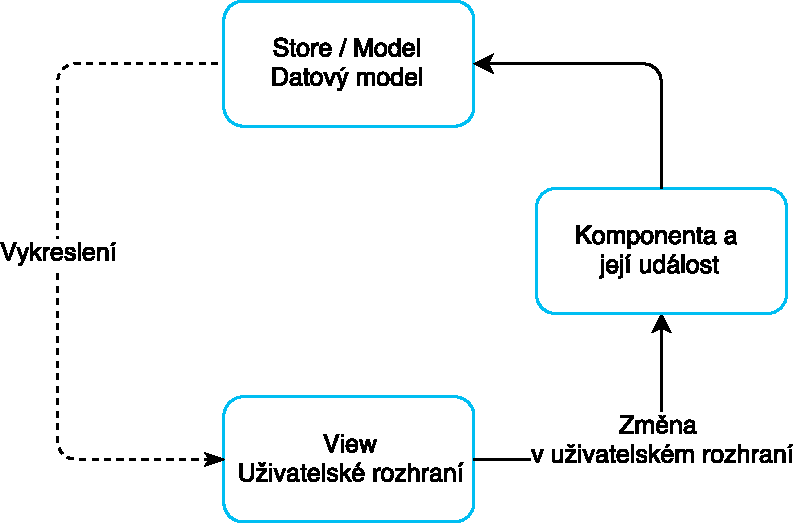
\includegraphics[width=11cm]{../OneWayDataBinding.pdf}
	\caption{Jednosměrný tok dat.}
	\label{fig:rctOneWayDataFlow}
\end{figure}

\subsection{Technologie serverových částí webové aplikace}
\label{sec:backend}

V této části diplomové práce budou popsány technologie serverových částí webové aplikace. Serverová část (backend) slouží nepřímo pro podporu front-endových služeb, obvykle tím, že je blíže k~požadovanému zdroji dat (databáze) nebo má schopnost komunikovat s~požadovanou databází. Zjednodušeně řečeno, jedná se o~část aplikace, která se odehrává mimo klientské stanice. Jakmile data opustí klientské prostředí a~doputuje na přístroj jiný, jedná se již o~backend. Cílem serverové části je například uchovávat data, provádět nad nima libovolnou logiku, vracet požadována data na základě požadavku, výpočty apod. v~následujících části si popíšeme technologii pro vývoj serverových částí aplikací, která byla použita v~praktické části diplomové práce. 

\subsubsection{.NET Web API}
\label{sec:dotNET}

.NET Web API\footnote{Application programming interface -- rozhraní pro programování aplikací. Shrňuje sbírku procedur, funkcí, tříd či protokolů nějaké knihovny (ale třeba i~jiného programu nebo jádra operačního systému), které lze využívat.} je framework od společnosti Microsoft pomocí kterého sestavujeme HTTP servisy, které dokážou obsluhovat příchozí požadavky jednoho či více klientů. .NET Web API je sada komponent, které zjednodušují programování HTTP. Výsledkem je, že webové rozhraní API je flexibilní a~snadno se rozšiřuje. Jazykem pro vývoji na tomto serverovém frameworku je C\#\footnote{Objektově založený jazyk od společnosti Microsoft.}. \\

\myparagraph{Domain Driven Design}

Pojem Domain Driven Design (dále jen DDD) byl poprvé zaveden v~roce 2004 Ericem Evansem v~jeho stejnojmenné knize. Doména v~tomto případě znamenám, že je to soubor společných požadavků, terminologie a~funkce pro libovolný program, konstruovaný k~vyřešení problému v~oblasti. Základem je, že návrh softwaru je silně ovlivněno oborem, pro který má být software vytvořen. DDD vyzdvihuje nutnost modelování objektů tak, aby tento model co možná nejvíce odpovídal reálné situaci. Snaží se tedy o~to, aby program byl modelem reálného systému nebo procesu. Při implementaci podle DDD úzce spolupracujeme s~odborníkem na doménu, který může vysvětlit, jak skutečný systém funguje. Pokud vyvíjíme informační systém v~nemocnici, může být doménovým expertem vrchní sestra. Mezi programátorem a~doménovým expertem se buduje všudypřítomný jazyk (ubiquitous language), což je jazyk, který popisuje koncept systému. Myšlenka je, že napsáno by mělo být to, co systém dělá způsobem, který odborník na doménu dokáže přečíst a~ověřit, že je správný. v~našem příkladu informačního systému bude všudypřítomný jazyk zahrnovat definici slov jako "pacient", "diagnóza", "léky" a~tak dále. Koncepty popsané v~UL (ubiquitous language) budou tvořit základ objektově orientovaného návrhu DDD poskytuje jasné pokyny o~tom, jak by měly objekty interagovat. Tento koncept architektury definuje na vysoké úrovni abstraktnosti jednotlivé doménové modely:\cite{19}

\begin{itemize}  
	\item \textbf{Entita} –- jedná se o~objekt s~jednoznačným identifikátorem. v~našem příkladě se jedná o~pacienta a~jeho identifikátorem je například rodné číslo. Tímto dokážeme rozlišit dvě entity od sebe. Tento základní stavební blok je datový objekt a~jedná se o~základní jednotkou informace. Pokud chceme v~aplikační vrstvě pracovat s~jakýmikoliv daty, která potom chceme ukládat do databáze, měníme instanci entity, nikdy neměníme data přímo. Entita definuje rozhranní, jaká data je možné uložit, změnit, získat.
	\item \textbf{Hodnotový objekt (Value object)} –- reprezentuje informaci, která nemá identitu. Zajímá nás pouze jeho hodnota a~ne konkrétně daná identita. Příkladem může být například již absorbovaná dávka rentgenového záření. Nezajímá nás konkrétní vyšetření ale pouze hodnota záření, kterou absorboval pacient. 
	\item \textbf{Agregát (Aggregate)} -- klastr objektů a~hodnotových objektů s~definovanými hranicemi kolem skupiny. Agregát zamezuje aby každý jednotlivý objekt (entita nebo hodnotový objekt) reagoval samostatně na externí podnět. Skupině objektů je přiřazen jednotlivá agregovaná kořenová položka. Nyní externí objekty již nemají přímý přístup ke každé jednotlivé entitě nebo hodnotovému objektu v~agregátu, ale místo toho mají přístup pouze ke kořenovému prvku s~jedním agregátem a~používají jej k~předávání pokynů skupině jako celku.
\end{itemize}

DDD také popisuje základní mechanismy:

\begin{itemize} 
	\item \textbf{Repozitář (Repository)} -- při práci s~entitami se očekává, že po restartu systému bude možné opět pracovat s~daty, které entita obsahovala. Je potřeba tedy mapovat data na entitu. Tento proces se v~relačních databází nazývá ORM (Object relational mapping). v~DDD se o~mapování dat z~datového úložiště na objekty stará tedy repozitář. Ať již vytváří objekty z~jakéhokoliv datového zdroje, vždy je prací repozitáře to, aby data převedlo z~konkrétního formátu na objekt se standardním rozhranním pro jejich zpracování – tedy na entitu. Repozitář je zodpovědný i~za ukládání dat – tedy převod entity na data ve formátu datového zdroje a~uložení těchto dat.
	\item \textbf{Služba (Service)} -- při analýze domény kdy definujeme hlavní doménové objekty může nastat chvíle kdy některé části domény nejsou jednoduše mapovatelné na objekty. Během rozhovoru programátora a~doménového experta vzniká všestranný jazyk, který popisuje základní principy domény, přičemž podstatná jména mohou prezentovat objekty a~slovesa jednotlivá interakce mezi nima. Mohou ale nastat případy kdy slovesa nelze tak snadno namapovat na žádnou interakci mezi objekty. V~tom případě je příhodné tuto funkci (interakci) definovat jako službu. Služby jsou vždy vystaveny jako rozhraní, nikoliv pro testovatelnost a~podobně, ale pro vystavení množin soudržných operací. Zjednodušeně pokud musí existovat nějaká funkce důležitá pro doménu, ale nemůže být spojena s~entitou nebo hodnotovým objektem, jedná se pravděpodobně o~službu.
	\item \textbf{Fabrika (Factory)} -- DDD navrhuje použití továrny, která zapouzdřuje logiku vytváření složitých objektů a~agregátů. Zajišťuje, že klient nemá znalosti o~vnitřním fungování objektů a~jejich logiku.
\end{itemize}

\section{Vlastní návrh řešení}

V této kapitole budou popsány detaily, které jsou nutné pro pochopení praktického řešení této diplomové práce. Budou popsány jednotlivé architektury, UML diagramy, technická řešení, fáze testování, proces nasazení, sbírání zpětné vazby i~retrospektivní zhodnocení. 

\subsection{Analýza současné situace}

Jak již bylo v~úvodu naznačeno (viz. kapitola \ref{sec:Uvod}) nedopadl předchozí pokus úspěšně. Toto řešení na míru bylo dodáno firmou Ekahau, která ovšem produkt zajišťující RTLS již na trh nedodává. Komunikace s~dodavatelskou firmou neprobíhala na uspokojivé úrovni a~firma nebyla schopná konzultovat vzniklé problémy v~provozu. Jelikož šlo o~black-box řešení, nešlo toto řešení modifikovat a~případně opravit. Proto byl navržen lokační systém v~reálném čase (Real Time Locating System~- dále jen RTLS), který zastřešuje ucelené řešení. Z toho důvodu, že je každá část v~plné režií, lze RTLS systém přímo naškalovat na požadavky zákazníka a~optimalizovat v~maximálně možném měřítku. V~konečném důsledku byl personál urgentního příjmu zatížen větší administrativou a~režií. Tato negativní zkušenost personálu pak hrála důležitou roli při definování požadavků a~detailnější pochopení chodu na urgentním příjmu Fakultní nemocnice Ostrava. Tato diplomová práce zajišťuje část tohoto uceleného řešení a~to měřící nástroj pro personál urgentního příjmu viz. obrázek \ref{fig:RTLS}.

\begin{figure} [H]
	\centering
	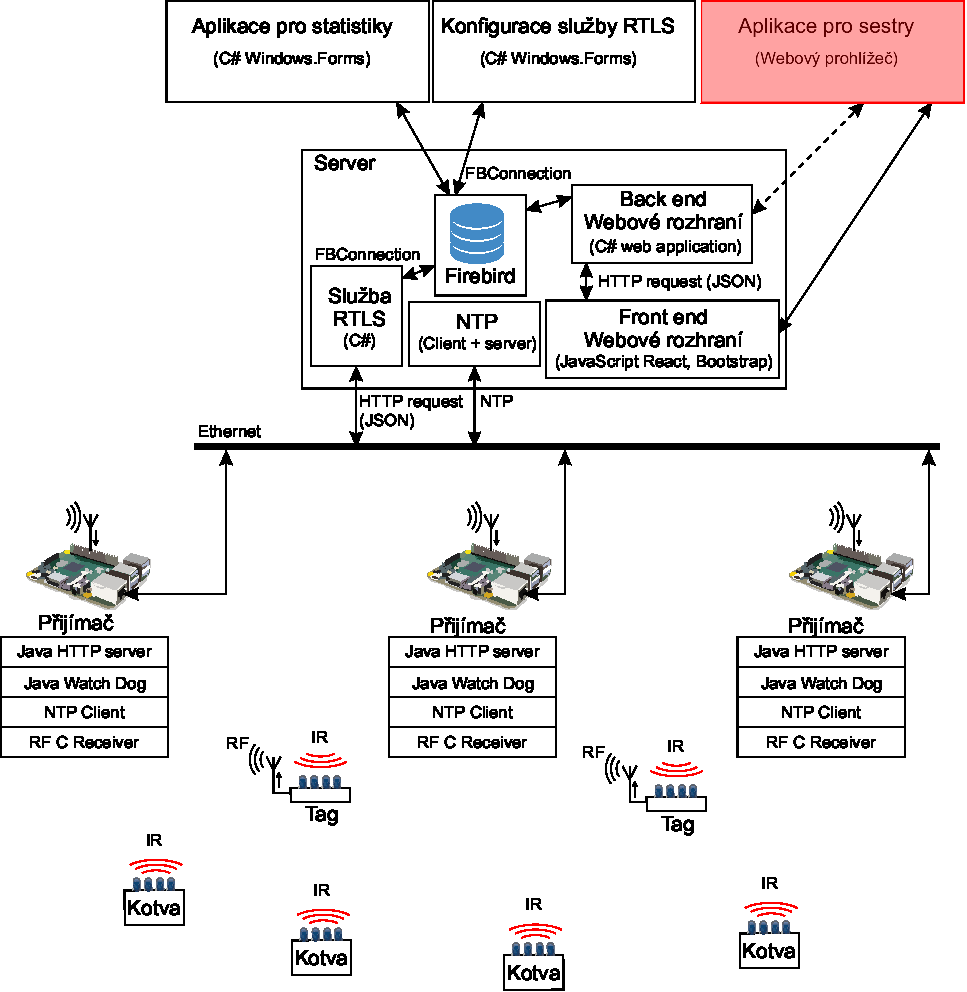
\includegraphics[width=15cm]{../RTLS.pdf}
	\caption{RTLS schéma. Kotvy jsou v~RTLS zařízení, které cyklicky vysílají do svého okolí informaci o~sobě. Tyto kotvy jsou umístěny v~každé místnosti minimálně jednou, vysílají pomocí infračerveného signálu informace o~tom, ve které budově se kotva nachází, místnost ve které je kotva umístěna a~roh místnosti. Předpokládá se maximálně 254 budov a~255 místností. Je nezbytné, aby na každé posteli pacienta byl přítomný tag. Lokalizační tagy jsou malá elektronická zařízení, která zajišťují lokalizaci v~hlídaném prostoru. Tagy sbírají data z~IR kotev a~v případě potřeb vyšlou potřebná data. Data jsou vysílána v~případě změně místnosti, zmáčknutí tlačítka na tagu nebo po uplynutí pěti minut po vysílání. Tato data jsou následně přijímána přijímači a~webovým serverem, který tato data zpracuje a~následně uloží do databáze. Tato centrální databáze pak obsahuje všechny události, které byly zaznamenány tagem. Toto úložiště dat pak využívá široká škála aplikací, konfiguračních nástrojů i~budoucí statistické vyhodnocování. Obrázek a~část textu převzata z~\cite{RTLS}.}
	\label{fig:RTLS}
\end{figure}
ekven
\subsection{Popis řešení}

Praktická část řešení vznikala od června roku 2017. Počátečním krokem bylo seznámení se s~doménou, doménovými experty a~uživateli. Bylo potřeba sesbírat požadavky a~informace o~tom, jak to na urgentním příjmu FNO funguje. Tento krok bývá v~procesu tvorby softwaru jeden z~nejdůležitějších. Pokud nejsou dostatečně prodiskutovány a~vymezeny požadavky, nemůže splňovat výsledný produkt očekávání zákazníka. \\

\myparagraph{Unified Modeling Language diagramy}

Unified Modeling Language (dále jen UML) je společný, sémanticky a~syntakticky bohatý vizuální modelovací jazyk pro architekturu, návrh a~implementaci komplexních softwarových systémů. Tento diagramový jazyk slouží pro rychlou orientaci, pochopení funkcionality a~chování systému. V~našem případě použijeme UML diagramy pro modelování funkcionalit (use case), které by měl systém umět. Komunikace byla pravidelná a~z rozhovorů vyplynulo, že je třeba upravit use case diagram. Na obrázku \ref{fig:UCDiagram1} je znázorněn UML diagram funkcionalit systému na základě požadavků urgentního příjmu FNO po první návštěvě. Na obrázku \ref{fig:UCDIagram2} je poté znázorněn konečný diagram funkcionalit.\cite{22}\\

\begin{figure} [H]
	\centering
	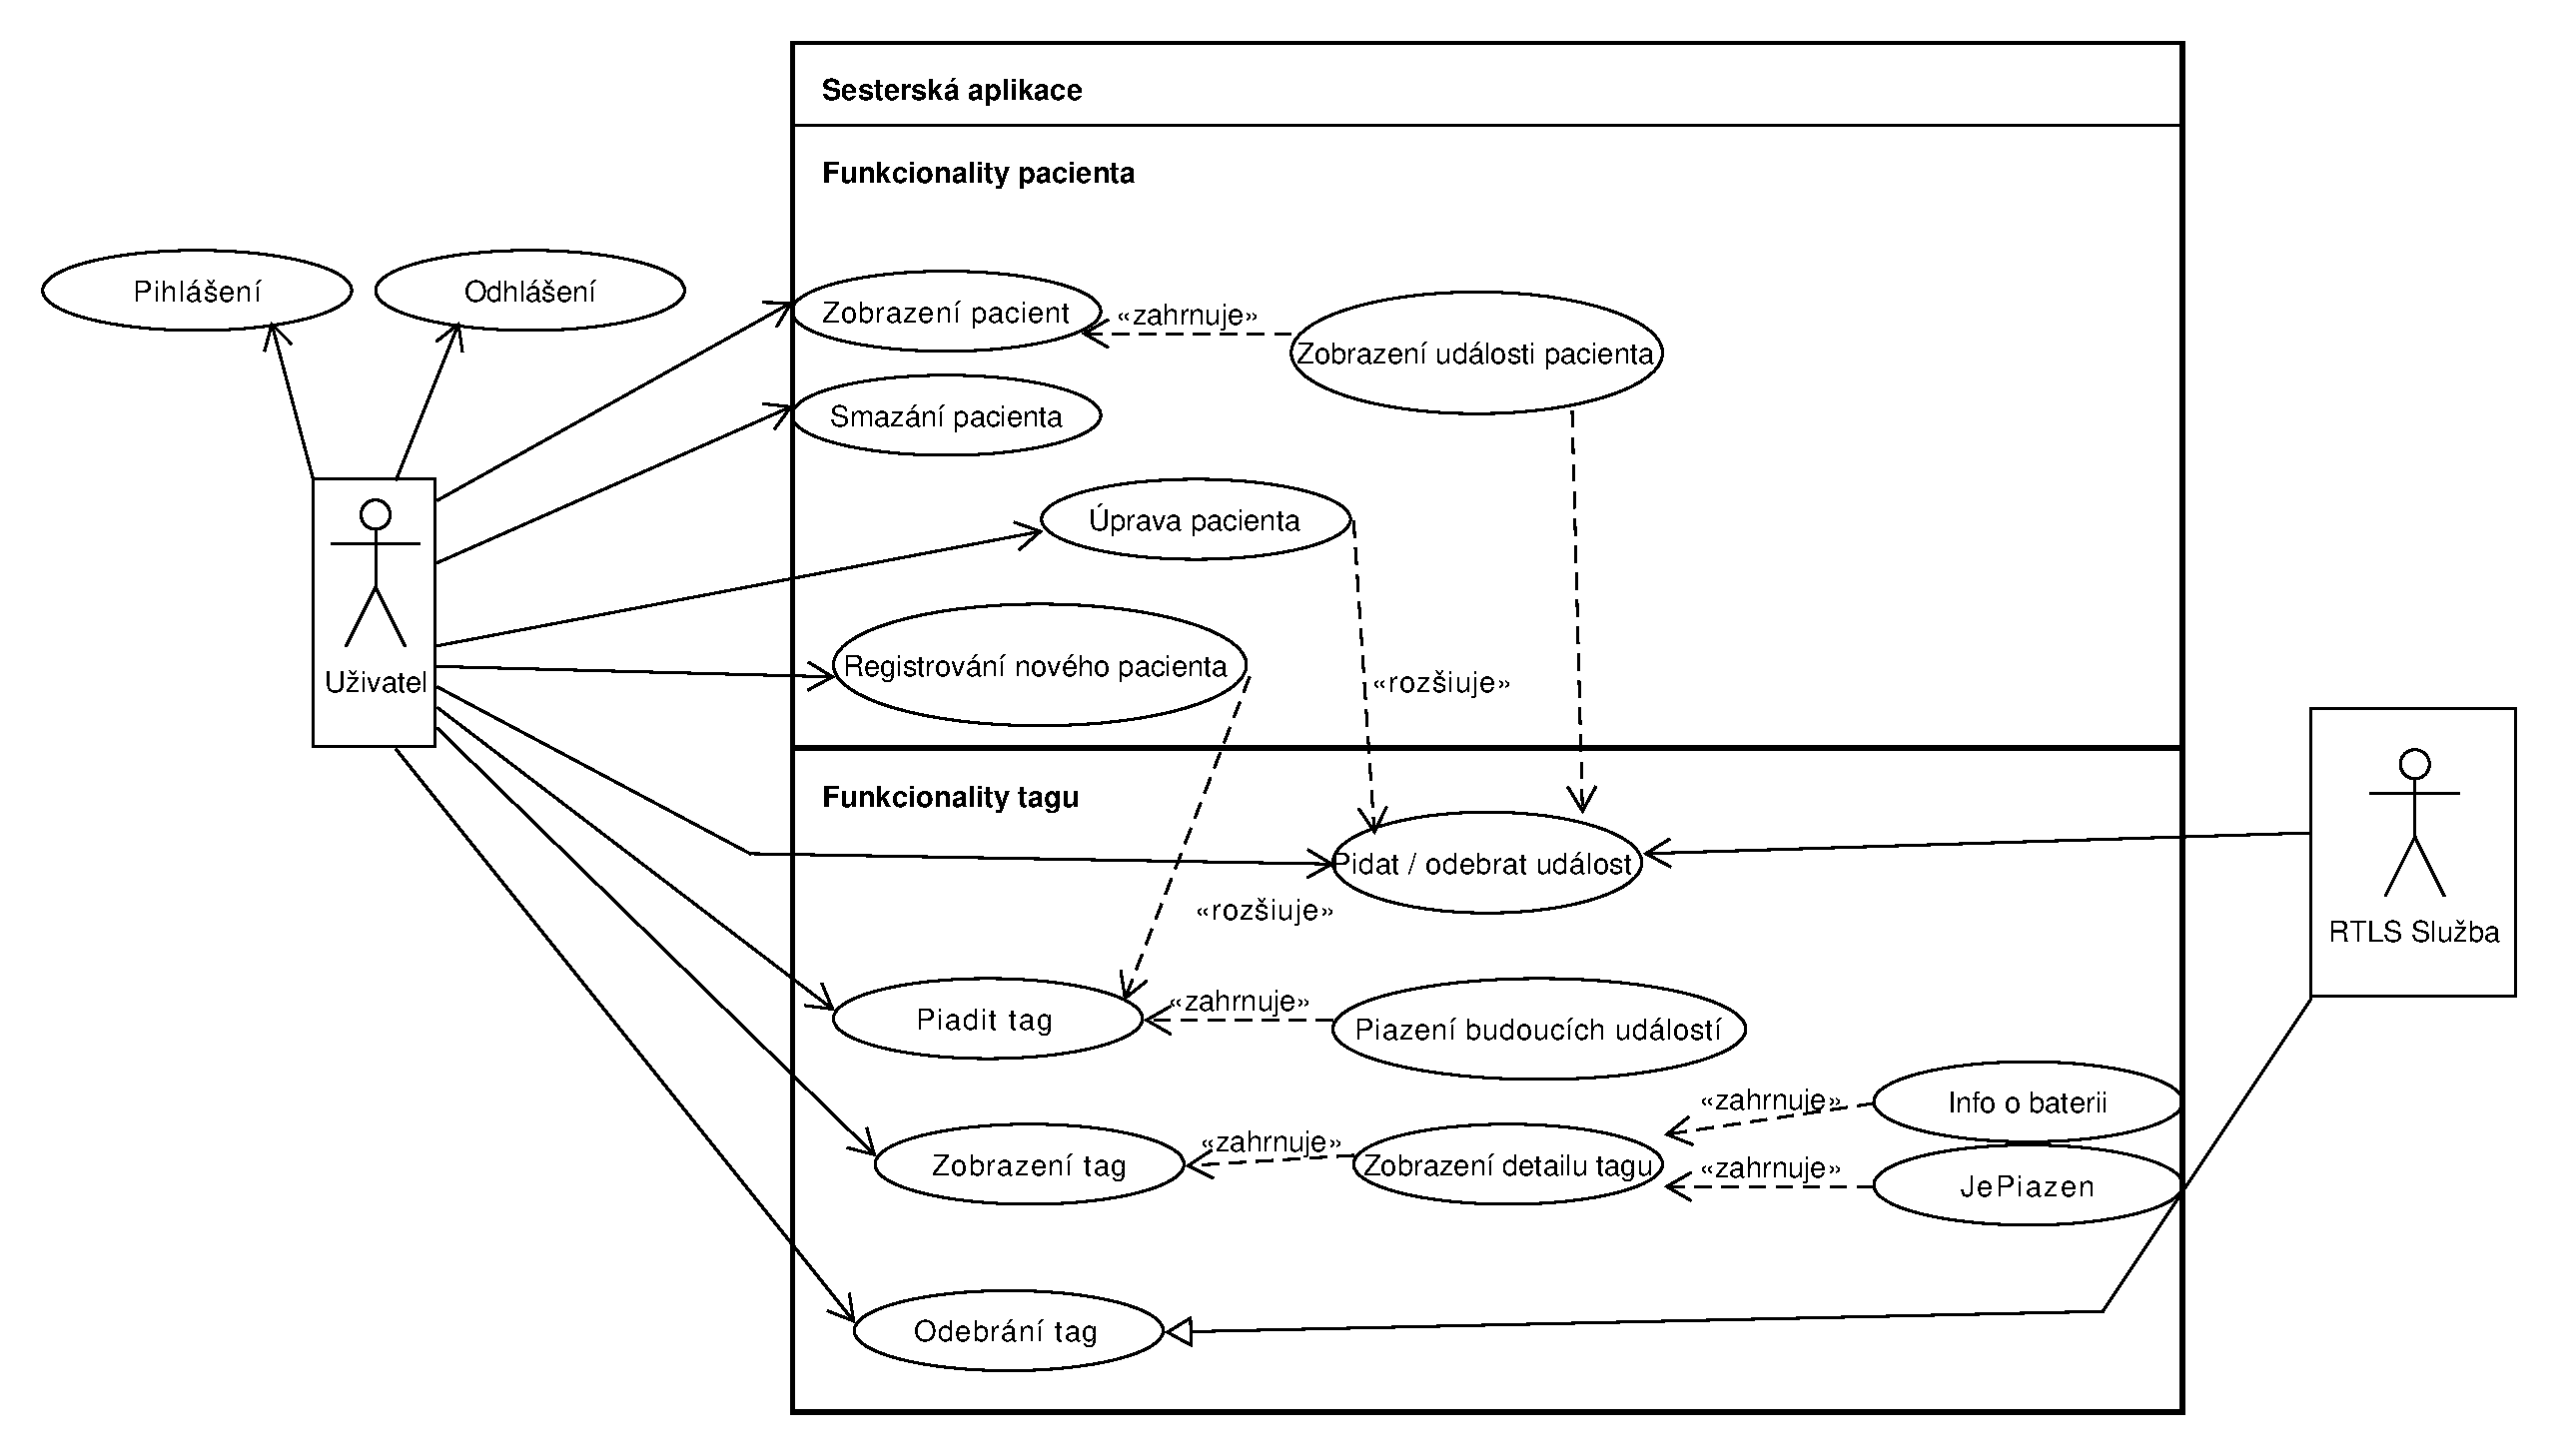
\includegraphics[width=15cm]{../UCDiagram1.pdf}
	\caption{Use case diagram po první schůzce.}
	\label{fig:UCDiagram1}
\end{figure}

\begin{figure} [H]
	\centering
	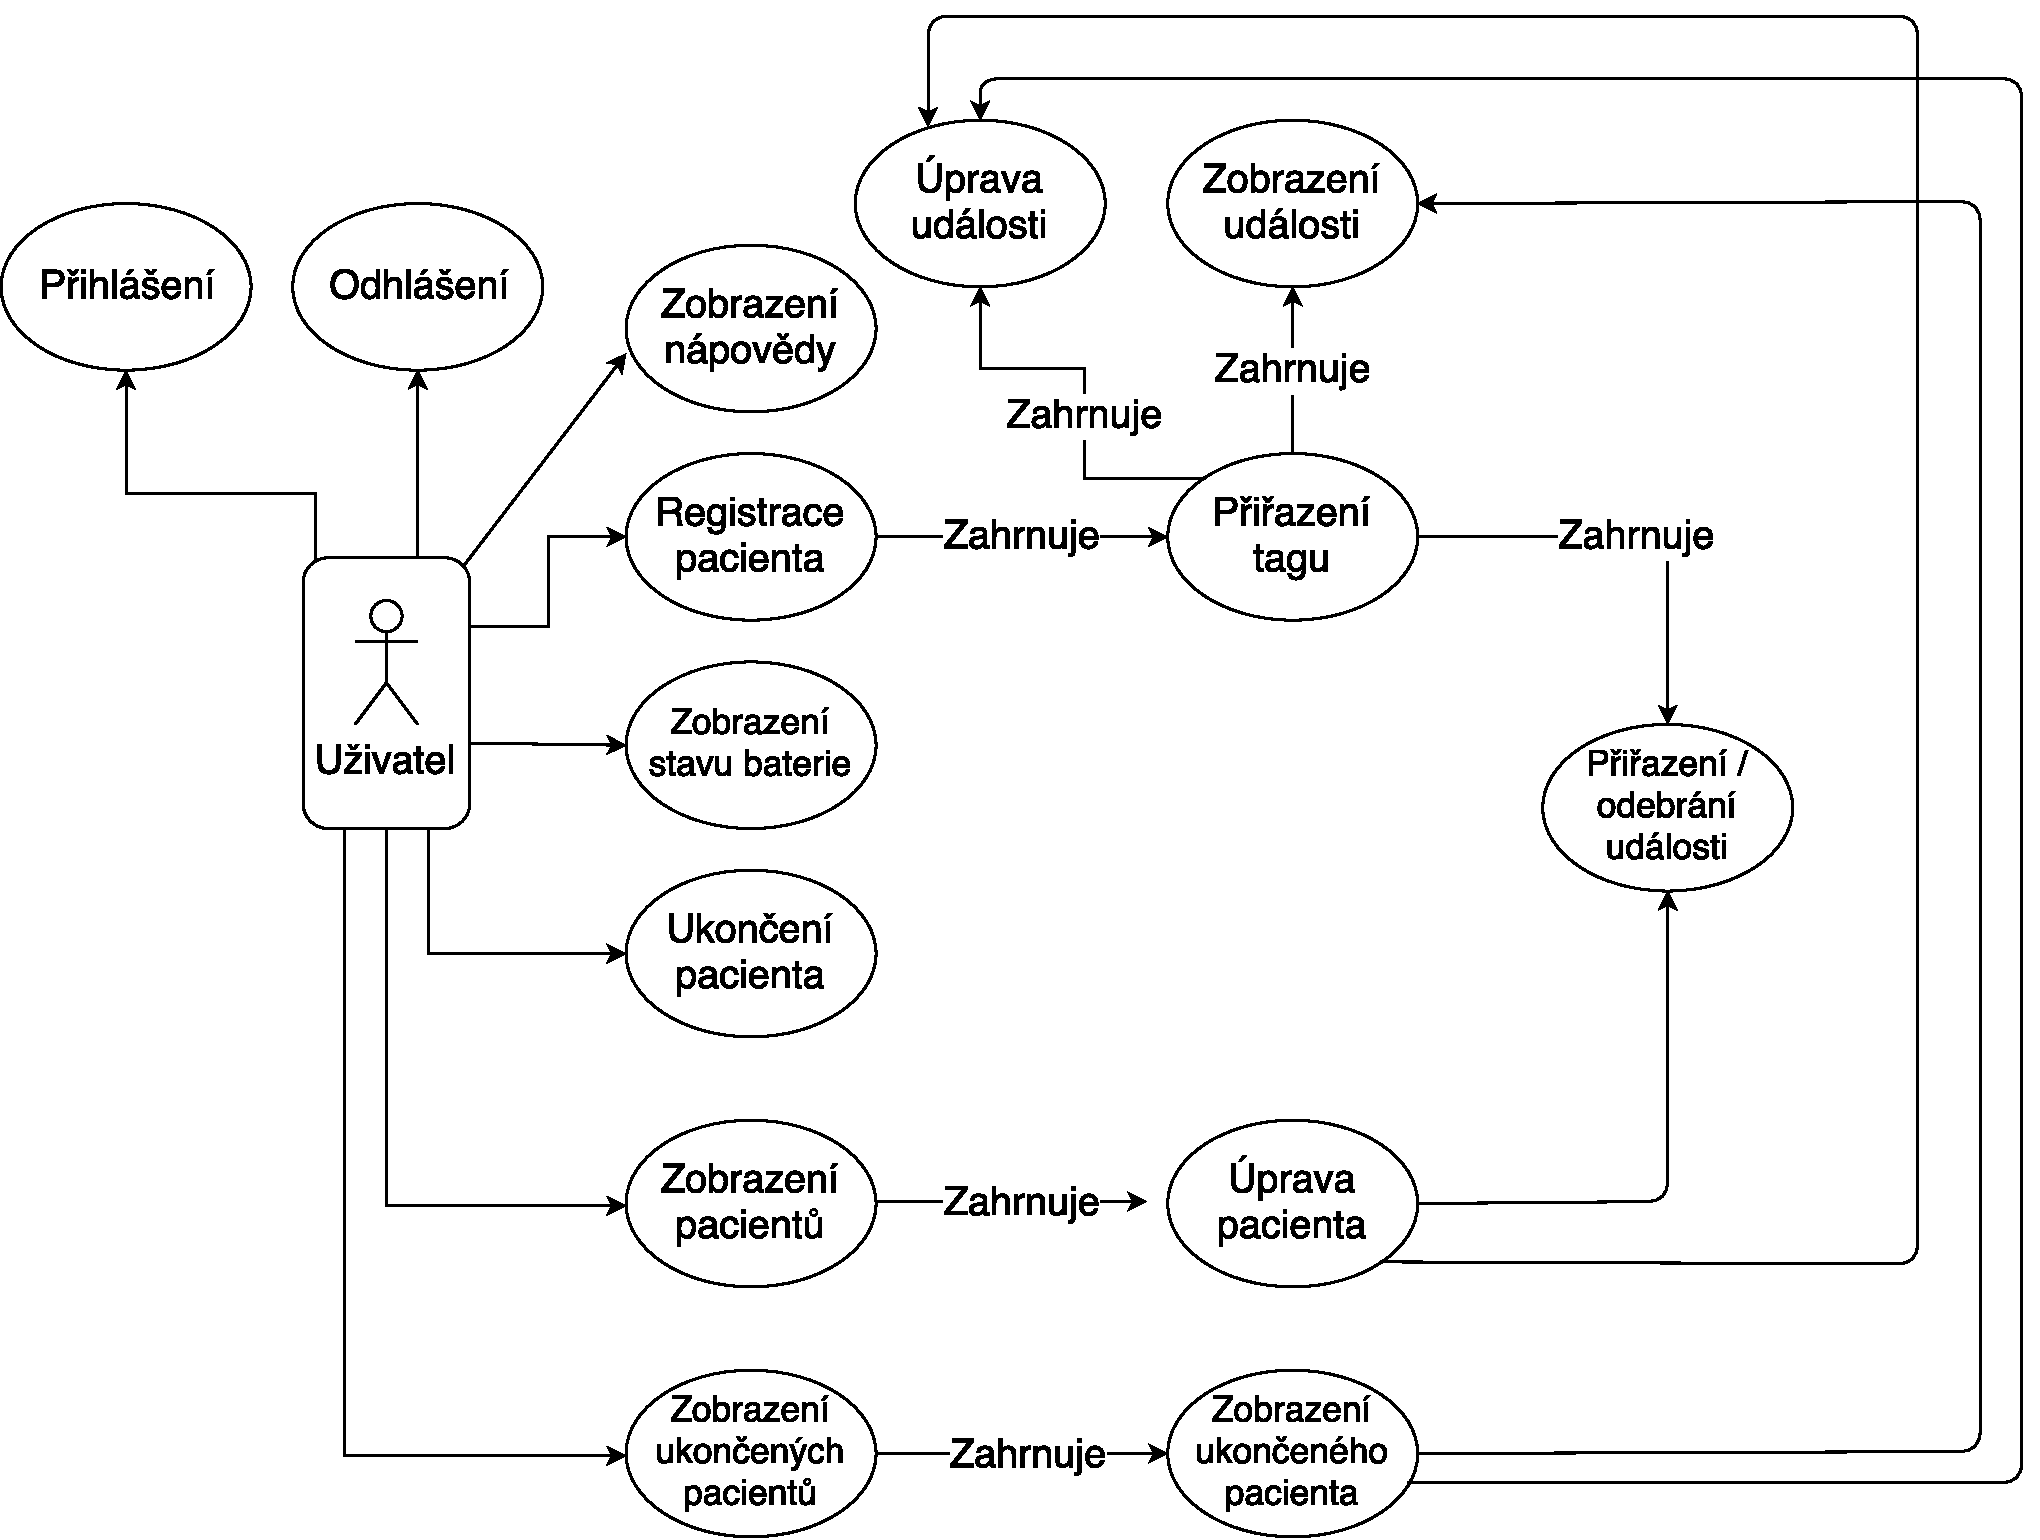
\includegraphics[width=15cm]{../UCDiagram2.pdf}
	\caption{Finální use case diagram.}
	\label{fig:UCDIagram2}
\end{figure}

Můžeme zpozorovat, že finální popis funkcionalit se od první verze značně liší. Některé aspekty byly zjednodušeny, některé zase naopak dodány. Po odsouhlasení use case diagramu lze pokračovat dále a~to je návrh uživatelského rozhraní. Finální popis funkcionalit viz. níže.

\begin{itemize}
	\item \textbf{Přihlášení do aplikace.}
	\item \textbf{Odhlášení z aplikace.}
	\item \textbf{Zobrazení nápovědy s~popisem funkcionalit.}
	\item \textbf{Registrace pacienta.} \\
		Vytvoření nového měření, kde se dodá číslo karty, což je povinný údaj nutný pro vytvoření měření. Nepovinné údaje jsou jméno, prostřední jméno, příjmení, rodné číslo a~datum narození. 
	\item \textbf{Přiřazení tagu.} \\
		Tento krok je obsažen pouze v~use casu registrace pacienta. Jedná se o~úkon, kdy je jednotlivému pacientovi přiřazen tag.
	\item \textbf{Úprava události.} \\
		K této funkcionalitě se lze dostat od přiřazení tagu, úpravy pacienta či zobrazení ukončeného pacienta. Jde o~úkon, kdy se upravují data události jako je čas či jeho název.
	\item \textbf{Zobrazení události.} 
	\item \textbf{Zobrazení stavu baterie tagu.} 
	\item \textbf{Ukončení pacienta (měření).} 
	\item \textbf{Zobrazení pacientů.}
	\item \textbf{Úprava pacienta.} \\
		Jde o~úpravu pacientových dat, práce s~jeho událostmi nebo úprava jednotlivých události.
	\item \textbf{Zobrazení ukončených pacientů.} 
	\item \textbf{Zobrazení ukončeného pacienta.}
	\item \textbf{Přiřazení / odebrání události.} \\
		Tento use case je o~správě události aktivního pacienta (měření). \\
\end{itemize}

\myparagraph{Návrh uživatelského rozhraní} 

Základní návrh (wireframe) byl bez režie ze strany klienta. Postup byl takový, že musel splnit všechny use casy (UC) z~UML diagramu (viz. obrázek \ref{fig:UCDIagram2}). Jak bylo uvedeno výše, UC se často měnil, doplňoval a~redukoval, z~toho vyplývá, že se poměrně hodně měnila i~wireframe aplikace. První návrhy aplikace jsou dostupné viz. příloha \ref{appendix}.

\myparagraph{Výběr technologického stacku\footnote{Výběr technologií ze kterých bude sestaven softwarový produkt}}

Dalším krokem v~praktické části bylo vybrat technologický stack technologií, který bude použit pro softwarové řešení pro správu pacientů a~tagů. Bylo potřeba zohlednit již hotové vrstvy (databáze), zkušenosti autora s~jednotlivými technologiemi, dlouhodobé trendy, podporu technologií, rychlost a~výkonnost aplikace. Po zralé úvaze byl nakonec tech stack vybrán následovně: \\

\begin{itemize}
	\item \textbf{Backend}~-- .NET Web Api\ref{sec:dotNET}
	\item \textbf{Frontend}~-- ReactJS\ref{sec:ReactJS} 
	\item \textbf{Databáze} (poskytnuta)~-- Firebird
\end{itemize}

\myparagraph{Technické řešení a~popis frontendové části} \\
V této podkapitole bude popsána detailněji frontendová část řešení. Jak bylo zmíněno výše, zvolenou technologií pro vývoj byl Javascriptový framework ReactJS. \\

\myparagraph{Babel} 

Jelikož byla tato práce psána v~EcmaScript 6 (ES6), který obsahuje funkcionality, které nejsou úplně všemi prohlížeči podporované, je potřeba překladače. Pro tyto účely byl vybrán Babel, který převádí Javascriptový zdrojový kód z~vyšších verzí do verze nižší. Pokud by kód nebyl přeložen a~tento kód by byl načten starší verzi prohlížeče, mohlo by se stát, že chování, vzhled nebo samotná aplikace bude nefunkční. Tento problém je nejvíce patrný u~prohlížeče Internet Explorer, který ani doposud nebyl schopen podporovat dnes již základní Javascriptové konstrukce.\cite{23} \\

\begin{lstlisting}[numbers=none, caption=ES6 kód využívající šipkového zápisu anonymní funkce., label=lst:ES6]
	patients.map(patient => console.log(patient.firstName));
\end{lstlisting}

\begin{lstlisting}[numbers=none, caption=ES6 kód po přeložení pomocí Babelu., label=lst:afterBabel]
	patients.map(function (patient) {
		return console.log(patient.firstName);
	});
\end{lstlisting}

\myparagraph{Webpack} 

Webpack je nástroj, který sdružuje velké množství zdrojových kódů do jediného souboru- bundle. Jelikož místo mnoha drobných JavaScriptových souborů je výsledný soubor jen jeden, je výsledná režie prohlížeče jednodušší a~rychlejší.\cite{21} \\

\begin{figure}[H]
	\centering
	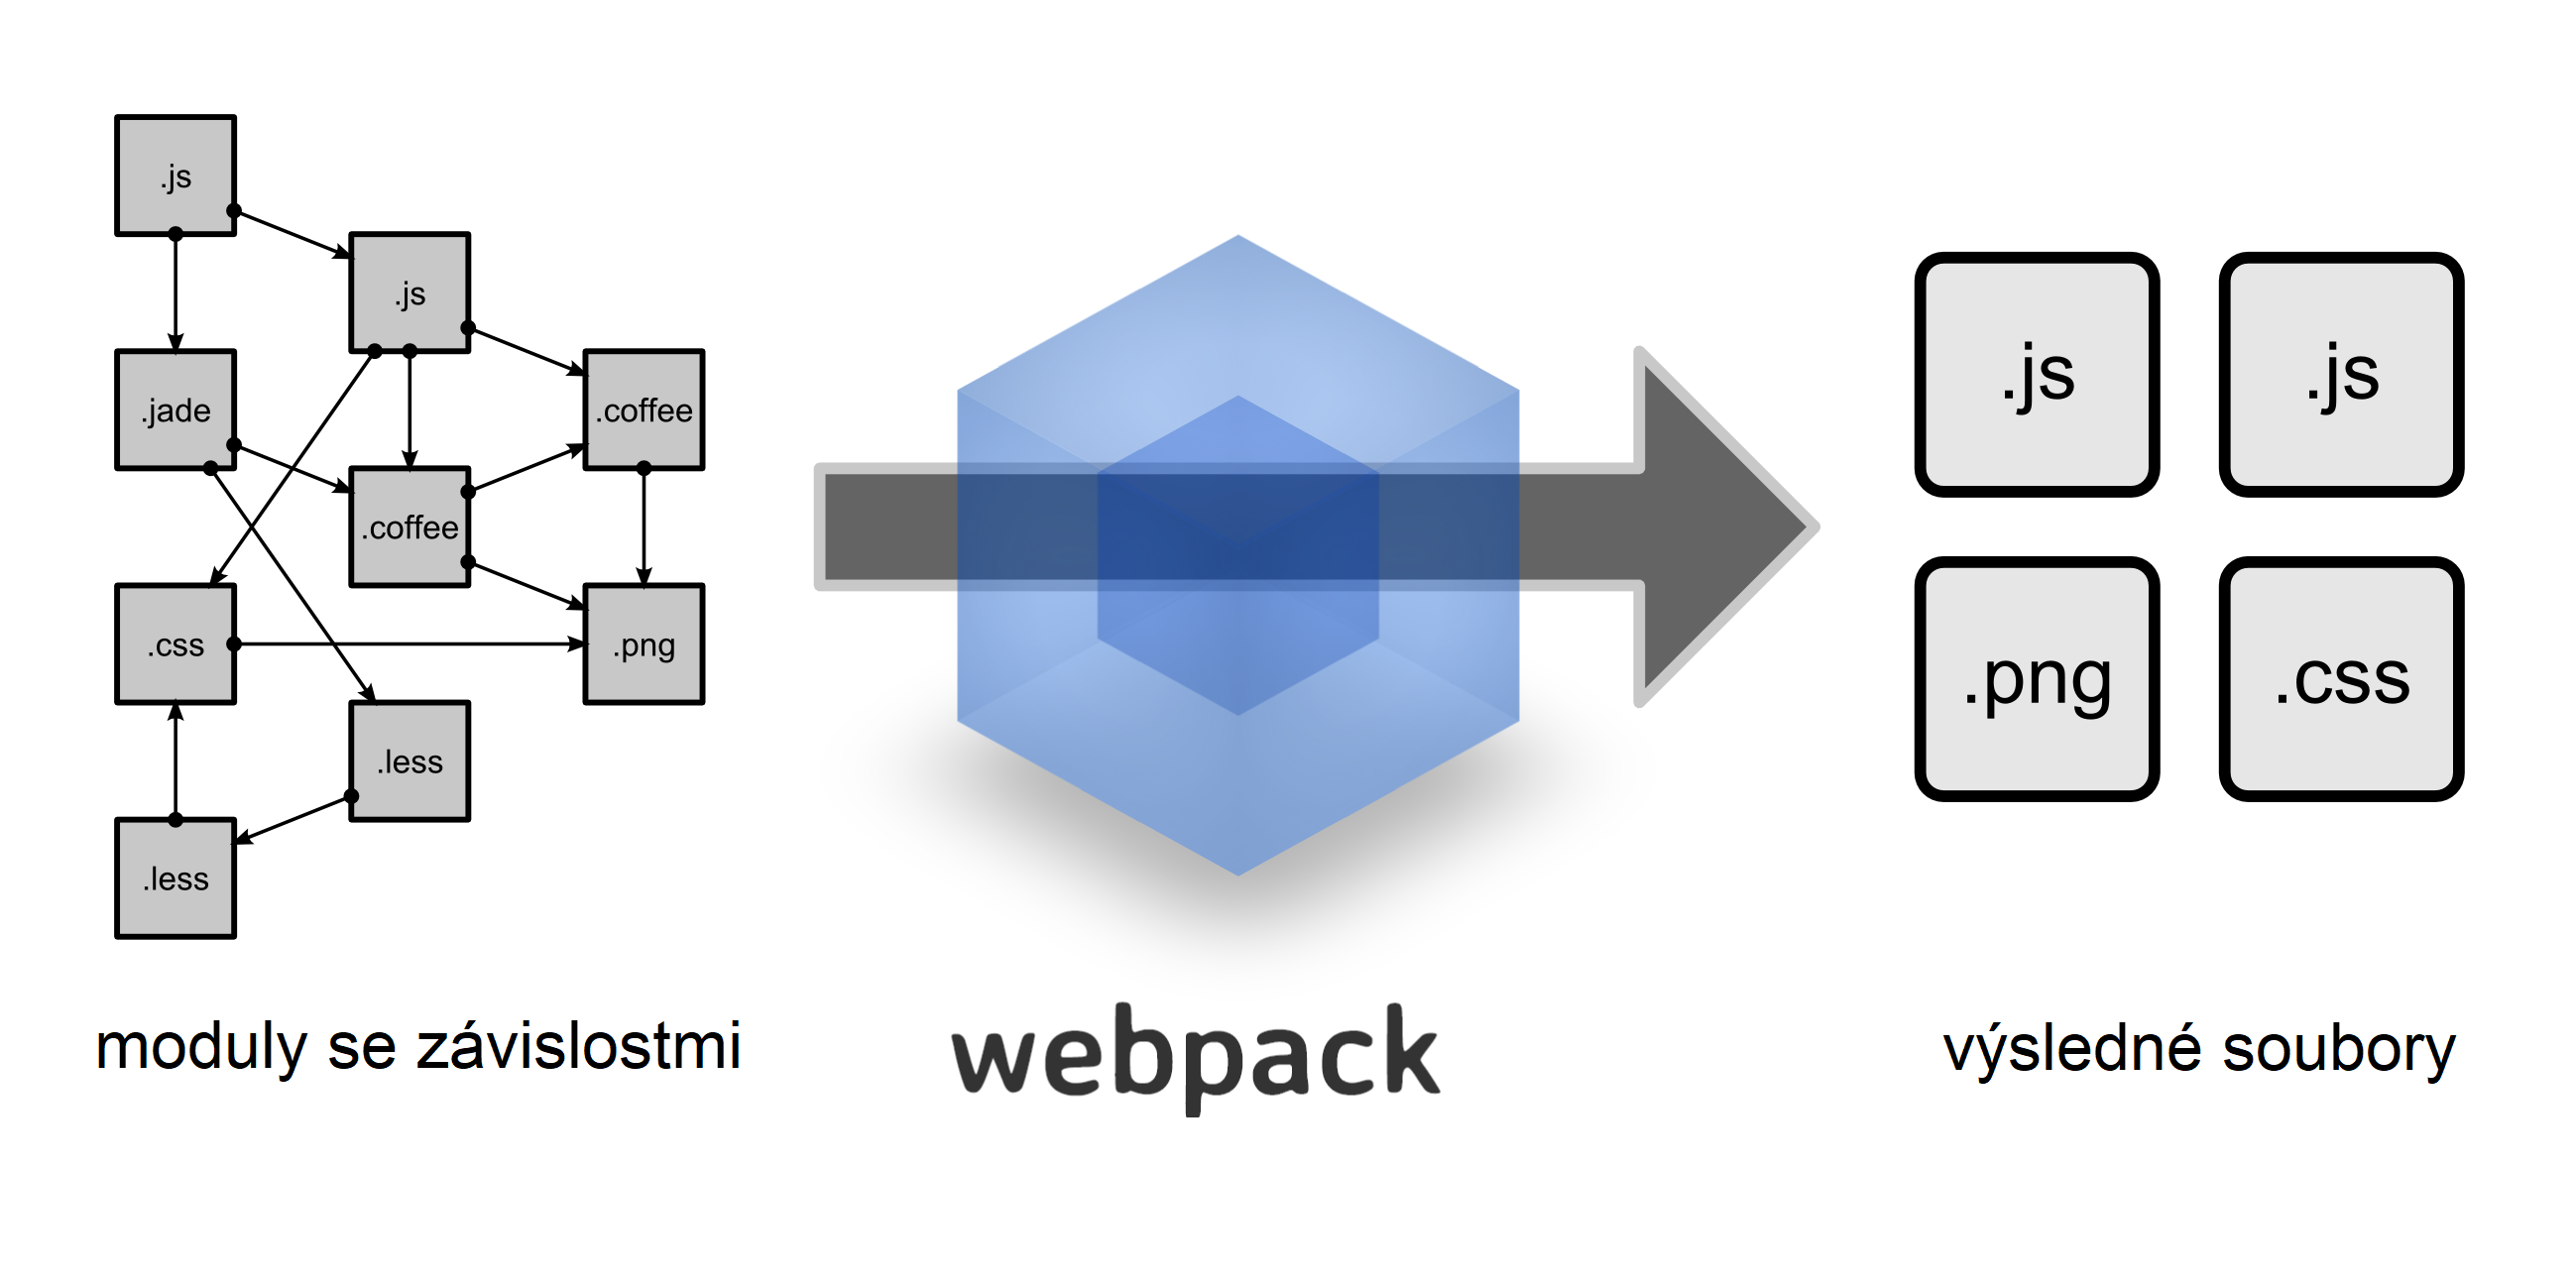
\includegraphics[width=15cm]{../webpack.png}
	\caption{Funkcionalita Webpacku. Převzato z~\cite{21}.}	
	\label{fig:Webpack}
\end{figure}

\myparagraph{Redux} 

Redux je knihovna, která se inspirovala knihovnou Flux od společnosti Facebook a~byla vytvořena v~roce 2015 Danem Abramovem. Redux může usnadňovat správu stavu (state) aplikace. Jinými slovy, pomáhá řídit tok dat, která jsou zobrazována, a~reaguje na akce uživatele. \\
Základní principy Reduxu jsou:

\begin{enumerate}
	\item Store je single-source-of-truth. (viz. \ref{sec:ReactJS}) \\
		Store celé aplikace je uložen v objektovém stromu v~jednom uložišti. Stav všech komponent aplikace závisí právě na onom objektovém stromu.
	\item Store je pouze v~módu čtení. 
		Nelze měnit store přímo z~View vrstvy.
\end{enumerate}

V Reduxu jsou pro práci se storem uzpůsobeny \textit{akce}, které se vysílají (dále jen dispatch). Tyto akce po dispatchnutí volají speciální funkce tzv. \textit{reduktory} (dále jen reducer), které následně modifikují store. Reducer si můžeme představit jako předdefinovaný objekt, který uchovává veškerá data části aplikace a~také operace, jak s~těmito daty pracovat.
 
Pro představu například \textit{PatientsReducer} obsahuje veškeré informace o~daných pacientech, jako je jejich jméno, příjmení, prostřední jméno, rodné číslo, číslo karty, datum narození apod. Dále~obsahuje operace pro práci s~těmito daty, jako je například \textit{ADD\_PATIENT}. Tyto operace mají určité požadavky a~omezení a~její konkrétní příklad bude dále popsán v~kapitole (viz. reducer operace).
Tento proces zobrazuje obrázek číslo \ref{fig:Redux}.

\begin{figure}[H]
	\centering
	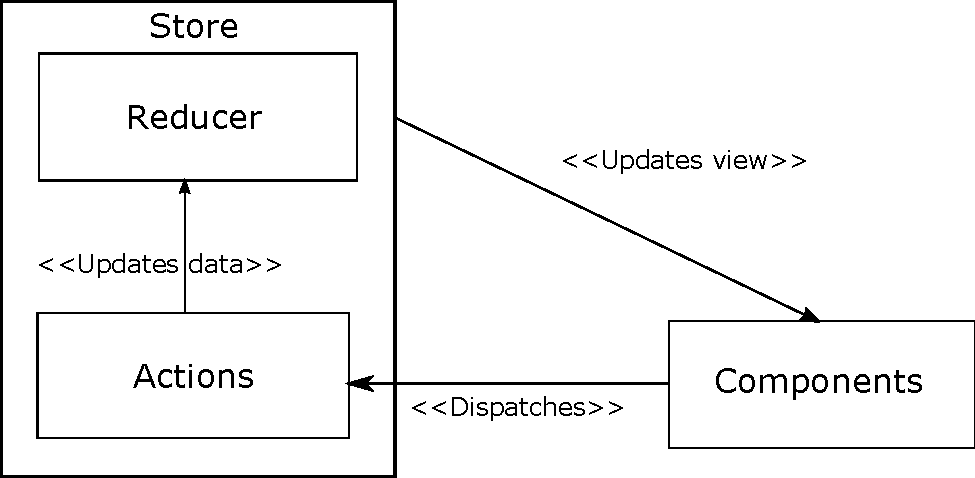
\includegraphics[width=15cm]{../Redux.pdf}
	\caption{Redux diagram}	
	\label{fig:Redux}
\end{figure}

Jak na obrázku vidíme, komponenty \textit{dispatchují akce}, které odchytí reducer a~aktualizuje data. Tato nová data jsou následně promítnuta zpět na komponenty, které se podle potřeby překreslí. \\

\myparagraph{Reducer operace} \\
Pokud chceme v~aplikaci změnit stav operace, musíme použít Redux. Redux obsahuje reducery, které se skládají z~dat a~operací, která modifikují data.

Data mohou být velmi jednoduchý objekt, jako je například následující výpis kódu. \\

\begin{lstlisting}[numbers=none, caption={Ukázka inicializačních dat v~reduceru pacienta.}]
const patientsInitialState = {
	patients : []
}
\end{lstlisting}

Operace pak reprezentuje jedna funkce, která přijímá dva argumenty. První argument je aktuální stav aplikace a~druhý je akce, která chce tento stav měnit.
Na typu této akce se pak rozhodne, která konkrétní operace se vykoná. Příklad této funkce lze vidět na následujícím výpisu kódu. \\

\begin{lstlisting}[numbers=none, caption={Reducer funkce}]
const PatientsReducer = (state = patientsInitialState, action) => {
	switch(action.type) {
		case 'ADD_PATIENT':    
		
			return { 
				...state,
				patients: [...state.patients, action.payload]
			}
		
		case 'FETCH_ACTIVE_PATIENTS':
			state.patients = action.payload
			return Object.assign({}, state);
		default:
			return state;
	}
}
\end{lstlisting}

Každý jednotlivý příkaz \textit{case} reprezentuje jeden typ akce, kterou lze s~daty vykonat.
Akce kromě svého typu nese ještě \textit{payload}, což jsou nová data. Je nutné si dát pozor, aby žádná akce nemodifikovala stávající stav,
ale vracela vždy kompletně nový objekt (immutable). O~toto se v~našem případě stará metoda \textit{Object.assign(\{\}, state, newData)}, kde první parametr značí, že se má vytvořit úplně nový objekt. \\

\myparagraph{React Bootstrap}

React Boobstrap je open-source frontendový framework pro rychlejší a~jednodušší vývoj webových aplikací. Obsahuje šablony návrhů založené na HTML a~CSS pro typografii, formuláře, tlačítka, tabulky, navigaci, modální okna a~mnoho dalších. Využitím tohoto frameworku lze zajistit správně reagující (responsive) aplikaci ve všech rozlišeních. React Bostrapobstrap je verze Bootstrapu, která byla přepsána do Reactu. Každá vlastnost je zde reprezentována React komponentou, kterou je potřeba nejdříve naimportovat. Je využívána napříč celou aplikací od jednoduchých tlačítek po složitější komponenty, jako jsou například modální okna. Příklad použití vidíme na výpisu \ref{lst:Bootstrap}.

\begin{lstlisting}[numbers=none, caption={Ukázka React Bootstrap}, label=lst:Bootstrap]
import { Button } from "react-bootstrap";

export default class Login extends React.Component {

	render() {
		return (
			<div className="Login">
				<Button bsSize="large" type="submit">
					Login
				</Button>
			</div>
		);
	}
}
\end{lstlisting}


\myparagraph{Technické řešení a~popis backendové části}

V této podkapitole bude popsáno technické řešení serverové části aplikace. Tato část byla implementována jako C\# Web API (viz. \ref{sec:dotNET}) využívající architekturu S\#harp, ORM systém NHibernate a~databázi Firebird. Tyto technologie budou popsány níže. \\

\myparagraph{S\#harp architektura} 

Architektura, která byla použita v~backendové části aplikace v~této diplomové práci je S\#harp. Jedná se o~architektonický základ pro rychlé vytváření udržitelných webových aplikací, který využívá .NET MVC s~NHibernate\footnote{Open source projekt, který mapuje například z~relačních databází na objektově relační v~.NET frameworku.} jako ORM. Staví na designu Domain Driven Design (viz. výše). Architektura jasně definuje následující vrstvy, přičemž nižší vrstva by neměla vědět nic o~té vrstvě vyšší. \\

Vrstvy jsou následující:

\begin{itemize}
	\item \textbf{Doména (Domain)} \\
	V této nejnižší vrstvě jsou obsažené doménové objekty. Entity, hodnotové objekty, vazby mezi objekty či doménové servisy sídlí v~této vrstvě. Doménová vrstva by měla být striktně nezávislá na jakýkolich vyšších vrstvách. Tato vrstva, která obsahuje doménovou logiku by tedy neměla vědět nic o~tom, jaký typ ORM je použit, v~jakém formátu data přicházejí či jaká technologie je použita pro uživatelské rozhraní. 
	\item \textbf{Infrastruktura (Infrastructure)} \\
	Vrstva infrastruktury nastavuje zdroje dat třetích stran. V~této vrstvě se například definuje způsob připojení (connection string) na databáze, volání do cizích API nebo načítání ze souboru. Tato vrstva umožňuje komunikovat s~externími systémy přijímáním, ukládáním a~poskytováním dat na vyžádání. V~této vrstvě je logika, která řeší integrování našeho systému s~externími systémy. Tato vrstva je závislá na doménové vrstvě a~zároveň je silně nezávislá na vrstvách vyšších.
	\item \textbf{Akce (Tasks)} \\
	Vrstva akcí nebo také vrstva aplikačních služeb. Její úlohou je propojení jakékoli nepodnikatelské logiky z~různých služeb třetích stran. Data, která jsou získána ve vrstvě infrastruktury jsou poslána vyšší vrstvě, kde dojde ke konkrétní úpravě výsledků na Data Transfer Object (DTO). Jedná se o~objekt, který vychází z~doménové vrstvy. Narozdíl ale od entity nebo hodnotového objektu obsahuje navíc nebo postrádá některé vlastnosti a~hodnoty. Jedná se tedy o~pomocný objekt, který se používá k~zapouzdření dat a~odesílání z~jednoho subsystému aplikace do jiného. Hlavní výhodou je, že snižuje množství dat, které je třeba odesílat mezi aplikacemi po síti. Představme si databázi pacientů, kde naše entita obsahuje ohromné množství vlastností (jméno, datum narození, rodné číslo, bydliště, obvodní lékař, poslední hospitalizace apod.) a~je vyvíjen backend pro statistické vyhodnocení vytíženosti jednotlivých ordinací. V~tomto případě nás nezajímá konkrétní údaje pacienta a~DTO bude tedy mnohem menší objekt než entita. V~této vrstvě by měly být nadefinované také jednotlivé překladače (mappers) mezi DTO a~doménovým objektem. Tento krok je zásadní pro škálovatelnost a~robustnost backendu. Mějme DTO objekt, který nám poslal klient, který obsahuje neúplné informace nebo data ve špatném formátu (např. chybějící číslo karty u~pacienta). Překládač tedy přeloží DTO objekt na entitu a~pokud chybí vlasnosti bez kterých například neuložíme do databáze, můžeme automaticky vrátit chybu. Tímto se zamezí zbytečné režií pro vrstvu infrastruktury. Tato vrstva je závislá na doméně a~infrastruktuře a~zároveň neví nic o~vrstvách vyšších.
	\item \textbf{Aplikace / Prezentace (Application / Presentation)} \\
	Tato nejvyšší vrstva obsahuje nejčastěji uživatelské rozhraní (pokud backend nějaké má), rozhraní pro správu nebo v~případě diplomové práce řadiče (controller). Jelikož je frontend zpracován jinou technologií a~hlavně je na straně klienta, rozhraní pro adminy není třeba a v~této vrstvě jsou tedy jen řadiče, které plní úlohu vstupních bodů do backendového systému. Tyto řadiče zpracovávají příchozí požadavky a~odesílají odpověď zpět volajícímu. V~této vrstvě se také mohou nacházet konfigurační soubory specifické pro aplikaci (číslo portu, cesty k~certifikátům, přístupové údaje apod.). Tato vrstva je plně závislá na všech spodních.
\end{itemize}

Cílem architektury (viz. obrázek \ref{fig:sharpArch}) je tedy oddělit jednotlivé vrstvy softwaru pro rozšířitelnost, škálovatelnost a~testovatelnost. Motivací je také rozbít aplikaci do funkčních bloků, které mají logickou závislost. Se správně rozvrženou architekturou tedy nemusíme předělávat celý software, pokud budeme migrovat například databázi. Stačí jen změnit vrstvu infrastruktury. Pokud nejsme spokojeni s~dosavadním rozhraním třetí strany, přepisujeme tedy pouze kód ve vrstvě akcí. V~reálném světě doména (obraz reality) zůstává pořád stejná v~nezávislosti na tom, jaké změny jsou na naší straně. Software by měl plně reflektovat požadavky domény a~pokud se doména změní, je třeba zavést změny ve všech vrstvách.\cite{20} \\

\begin{figure} [H]
	\centering
	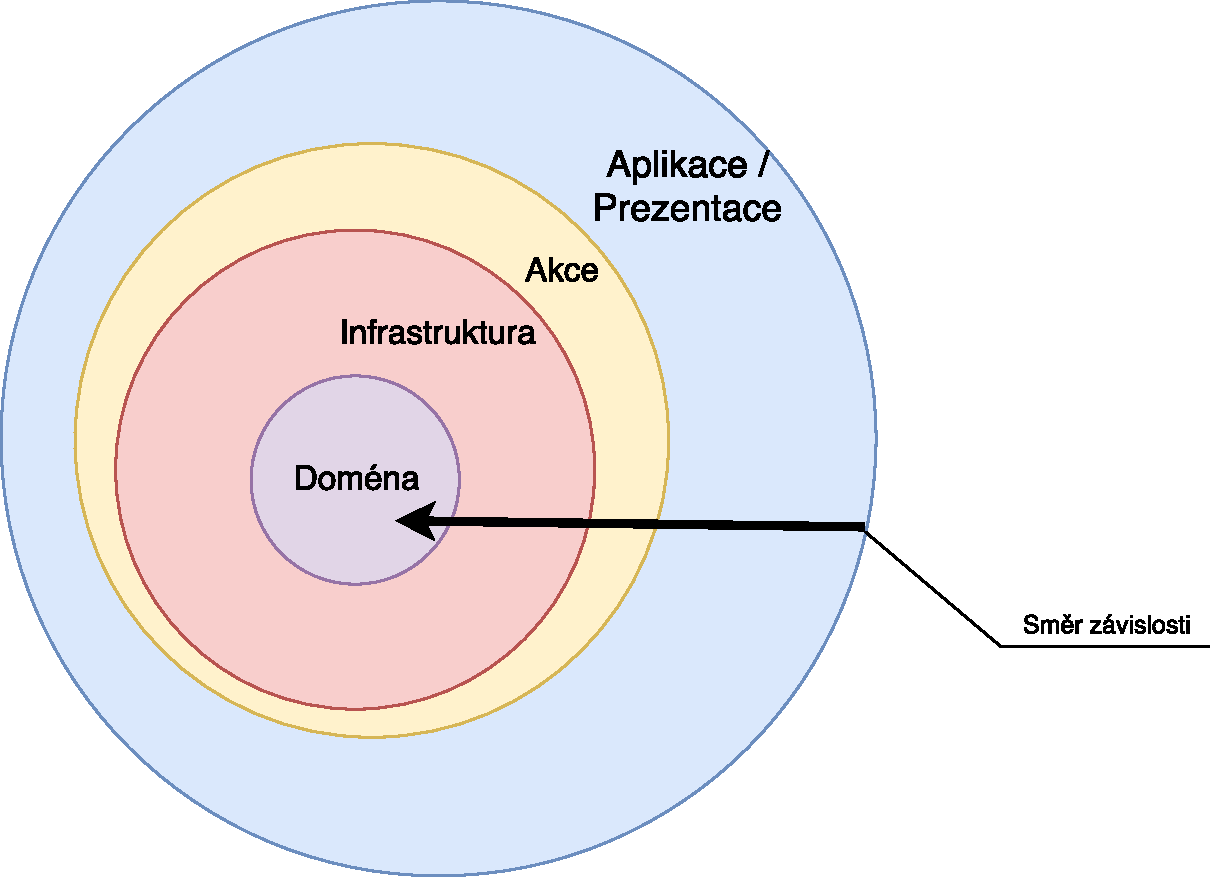
\includegraphics[width=13cm]{../SharpArchitecture.pdf}
	\caption{Rozvrstvení aplikace podle S\#harp architektury a~ukázka závislosti.}
	\label{fig:sharpArch}
\end{figure}

\myparagraph{NHibernate}

NHibernate je knihovna pro objektové modelování relačních databází (Object Relational Mapping dále jen ORM) určená pro použití v~.NETu. Tyto ORM vrstvy jsou zde z~toho důvodu, že neexistuje snadné spojení mezi objektovým a~databázovým světem. v~objektovém světě se vše točí kolem objektů, které drží informace o~datech. v~databázovém světě se data ukládají do tabulek a~jednotlivé objekty jsou reprezentovány řádky a~jeho vlastnosti pak sloupcemi. V~tomto řešení byla nad touto NHibernate knihovnou ještě naimplementována knihovna FluentNHibernate, která eliminuje úmorné ruční mapování pomocí rozsáhlých XML dokumentů (viz. \ref{sec:KlientServer}). Na základě nadefinovaných konvencí pro FluentNHibernate dokáže tato nadstavba nad ORM vrstvou nabídnout časově a~kódově úspornou alternativu ke standartnímu mapování v~NHibernate. Konvence můžeme psát v~C\# jazyce, což zlepšuje čitelnost, debugování a~refaktorovatelnost. Dalším důvodem je, že kompilátor nám nehlídá obsah XML dokumentu a~snadno tedy může docházet k~typografickým chybám, kdy se zamění názvy proměnných nebo vlasností objektů. Na výpisu \ref{lst:FluentNHibernate} vidíme příklad použití mapování.\cite{24}

\begin{lstlisting}[numbers=none, caption={Ukázka mapování pomocí FluentNHibernate}, label=lst:FluentNHibernate]
	public class PatientOverride : IAutoMappingOverride<Patient>
	{
		public void Override(AutoMapping<Patient> mapping)
		{
			mapping.Cache.ReadOnly().Region("LongTermReadWrite");
			mapping.Id(x => x.Id).GeneratedBy.Sequence("GEN_PATIENT_ID");
			mapping.HasOne(patient => patient.Tag).Not.LazyLoad().Cascade.All(); 
		}
	}
\end{lstlisting}

Další funkcí NHibernatu je poskytnutí metod pro vykonávání dotazů nad databází. Generuje dotazy v~Hibernate Query Language (dále jen HQL), což je dotazovací jazyk na nižší úrovni. Pomocí nastavení dialektu dokáže tedy přeložit různé syntaxe (MS SQL, MySQL, Oracle, PostgreSQL, SQLite, Firebird) dotazovacích jazyků do jednoho univerzálního HQL jazyka. NHibernate také zajišťuje správu a~mapování dědičností a~vazeb do databázové světa ve formě primárních a~cizích klíčů. Dále, jak je vidět na výpisu, \ref{lst:FluentNHibernate} využívá NHibernate i~cachování dat. Caching je proces, kdy se data ukládají do dočasného místa v~paměti, která jsou rychle dostupná. Caching se obnovuje, pokud jsou data změněná. \\

\myparagraph{Firebird}

Firebird je open-source multiplatformní relační databáze, která vznikla z~InterBase databáze v~roce 2006. Jelikož návrh databáze vzniknl dřív, byla tato databáze společně se schématem již poskytnuta. Pro účely tohoto řešení byly navíc vytvořeny tabulky \textit{Patient} a~\textit{User} společně s~generátory pro tvorbu ID. Databázové schéma je na obrázku \ref{fig:db}. \\
%TODO: doplnit db schema

\begin{figure} [H]
	\centering
	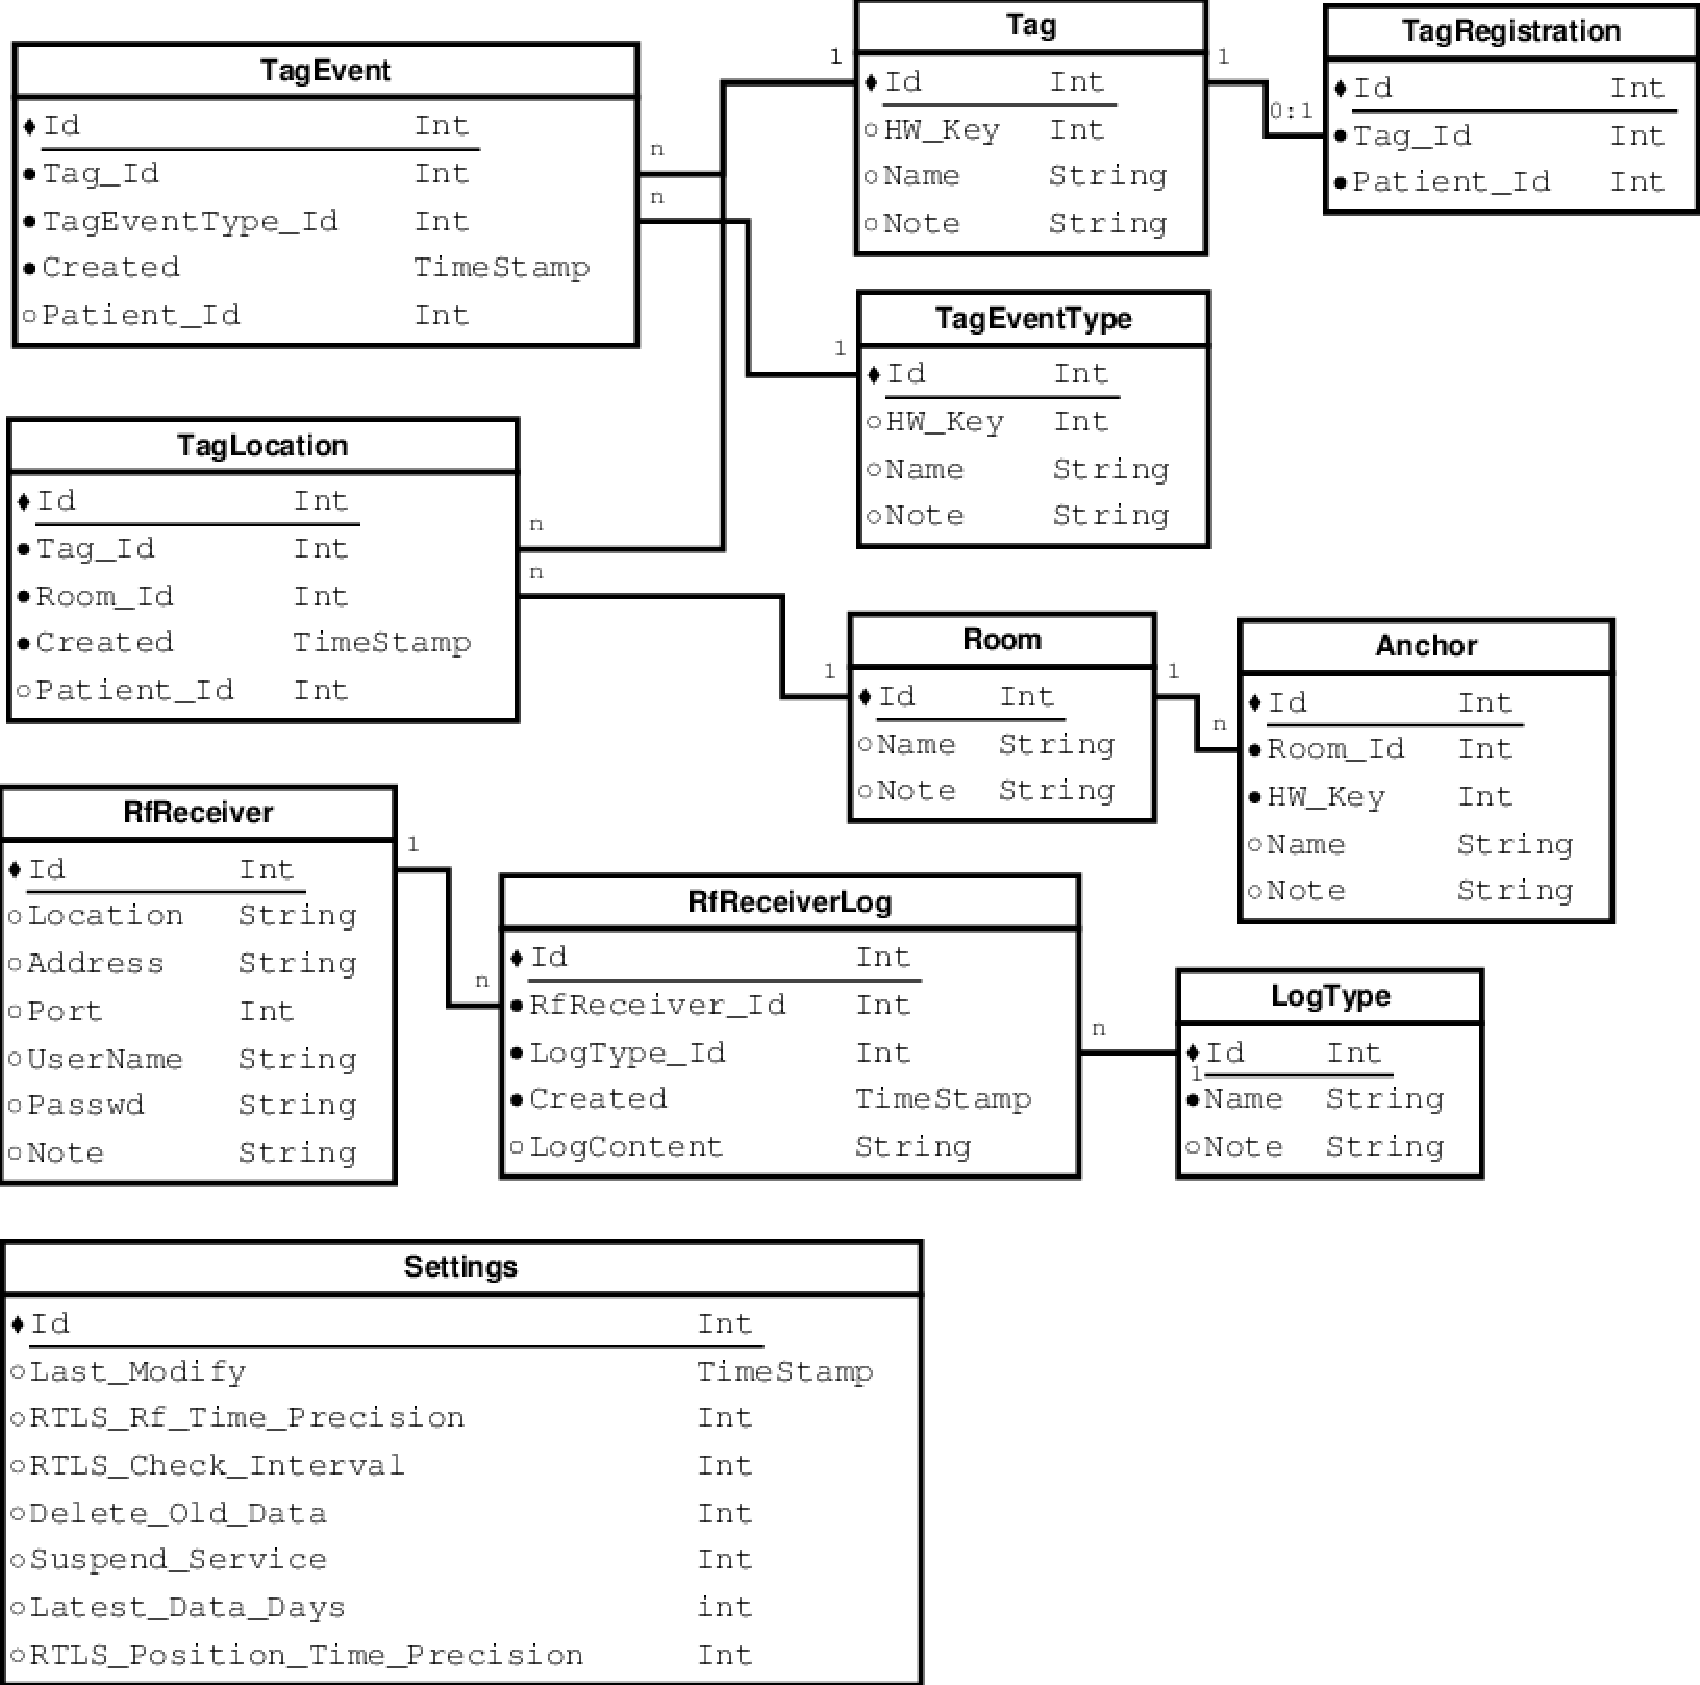
\includegraphics[width=14cm]{../databaze.pdf}
	\caption{Schéma RTLS databáze.}
	\label{fig:db}
\end{figure}

WebAPI rozčleněno podle S\#harp architektury znázorněno na obrázku \ref{fig:WebAPISolution}

\begin{figure} [H]
	\centering
	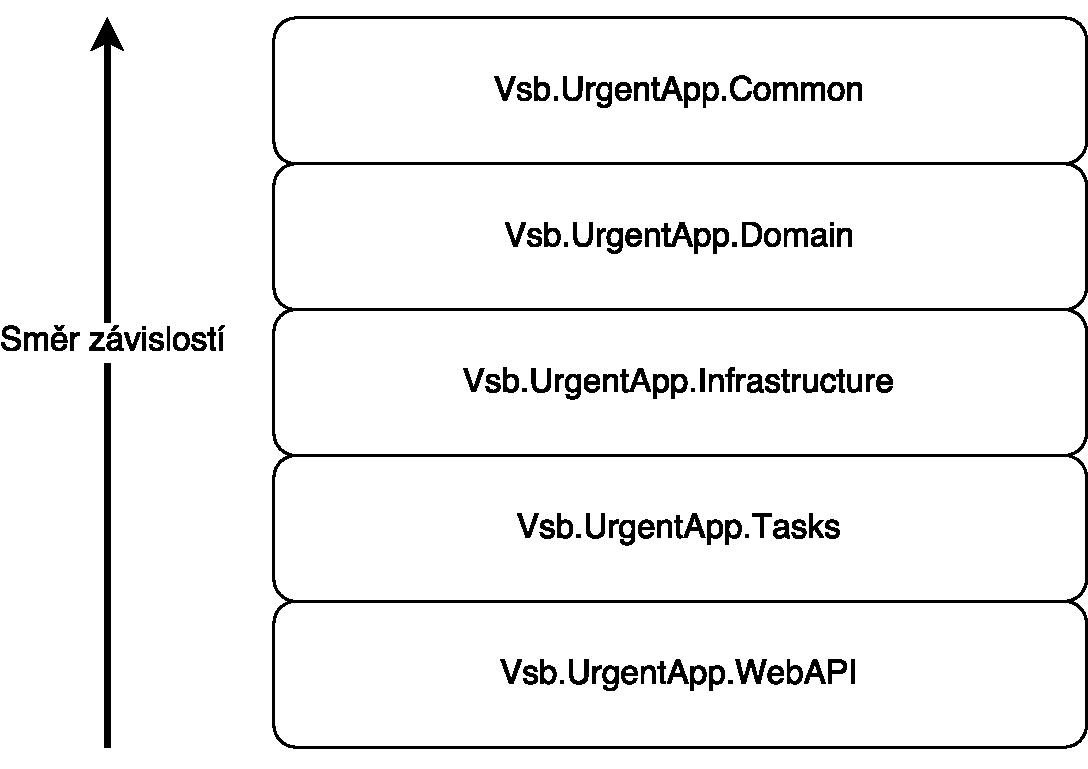
\includegraphics[width=10cm]{../WebAPISolution.pdf}
	\caption{Implementace backendu podle S\#harp architektury.}
	\label{fig:WebAPISolution}
\end{figure}

Na obrázku \ref{fig:SequenceDiagram} je znázorněn sekvenční diagram vytvoření pacienta. Tento diagram je pouze zjednodušený obrázek těch nejzásadnějších operací, které se dějí mezi danými participanty. \\

\begin{sidewaysfigure}
	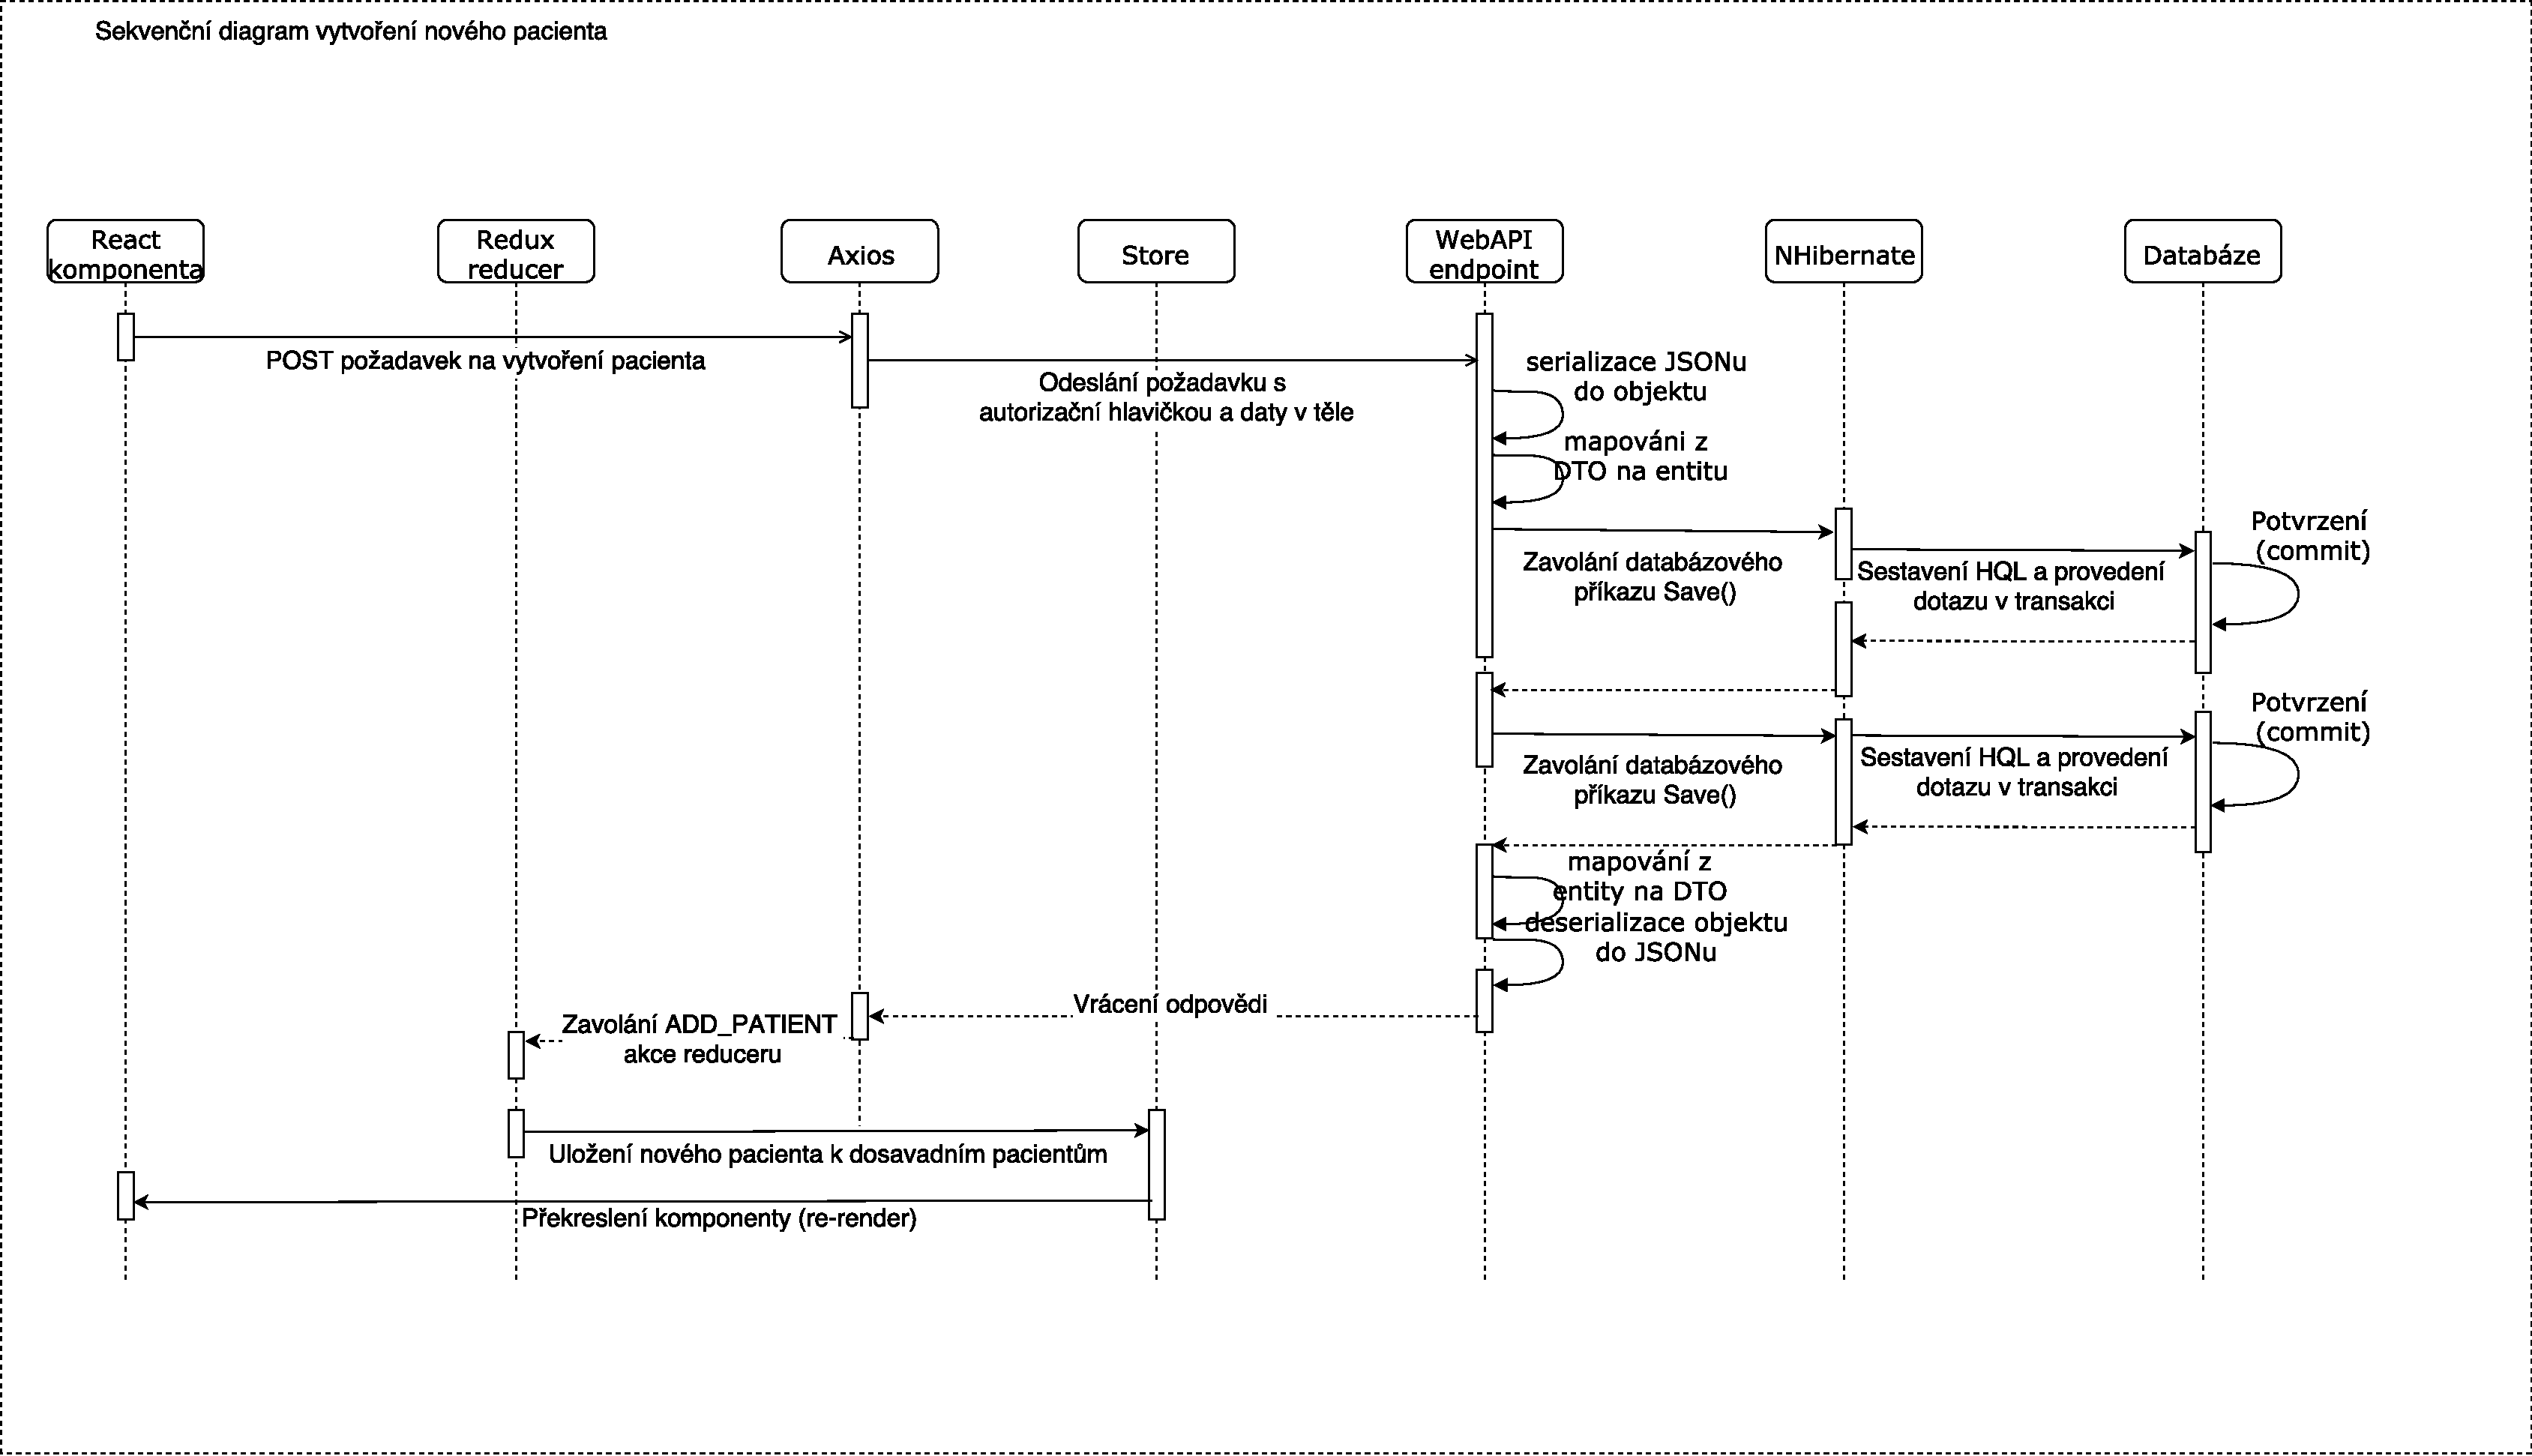
\includegraphics[width=22cm]{../SequenceDiagram.pdf}
	\caption{Sekvenční diagram vytvoření pacienta.}
	\label{fig:SequenceDiagram}
\end{sidewaysfigure}

\myparagraph{Kompilace}

Tato kapitola bude pojednávat o způsobu sestavení všech částí programu nutných pro úspěšné spuštění aplikace. V prvé řadě je nutné nainstalovat následující nástroje:

\begin{itemize}
	\item .NET kompilátor (obsažen ve Visual Studio)
	\item NodeJS + NPM (doporučená verze 6.10.1)
\end{itemize}

Řešení se dělí na složku \textit{backend}, která obsahuje zdrojové kódy z backendové části a \textit{frontend}, která zase obsahuje zdrojové kódy frontendové části. Pro zkompilování souborů backendové části nám pouze stačí vývojové prostředí Visual Studio (viz. \ref{sec:nastroje}), které obsahuje integrovaný .NET kompilátor. Tento nástroj nám poté zakompiluje soubory (přípona \textit{.cs}) do dynamických linkovaných knihoven (Dynamic Link Library dále jen DLL). Tyto soubory se nachází v cestě \textit{backend\textbackslash Vsb.UrgentApp.UI\textbackslash Vsb.UrgentApp.API\textbackslash bin}. Backend obsahuje ještě jeden projekt, který obsluhuje požadavky pro získání html souboru (který obsahuje styly a zabundlovaný JS soubot viz. \ref{sec:HTML} a \ref{sec:ReactJS}). Proces kompilace je stejný jako u API projektu a DLL soubory se nachází v \textit{backend\textbackslash Vsb.UrgentApp.UI\textbackslash Vsb.UrgentApp.UI\textbackslash bin}. V případě, že nejsou staženy závislosti knihoven třetích stran, je potřeba přes Nugget Manager obnovit tyto knihovny v případě, že selže automatický proces inicializace Visual Studia. 

Sestavení frontendu je trochu složitější. Zaprvé je nutno v adresáři \textit{frontend} spustit příkaz \textit{npm install}, kterým stáhneme všechny externí zavislosti, které jsou nadefinovány v souboru \textit{package.json}. V tomto souboru je také závislost na Webpack, který se tímto příkazem nainstaluje také, ale je jej potřeba nainstalovat také globálně. Globální instalace je potřeba, aby byl příkaz \textit{webpack} dostupný v~příkazové řádce, aby mohl být spouštěn pomocí skriptů. Této globální instalace docílíme spuštěním příkazu \textit{npm install webpack@3.8.1 -{}-global}. Dále- ve stejném adresáři je potřeba spustit příkaz \textit{npm run build}, který pomocí webpacku sestaví výsledný JS soubor a zároveň s pomocí Babelu převede na verzi, které rozumí i starší webové prohlížeče. Tento výsledný JS soubor poté vloží do \textit{backend\textbackslash Vsb.UrgentApp.UI\textbackslash Vsb.UrgentApp.UI\textbackslash built }, kde je narefencován v HTML souboru.


\subsection{Testování, nasazení a~zpětná vazba}

\myparagraph{Testování}

Testování softwaru je proces vedoucí k~informování zúčastněných stran o~kvalitě softwarového produktu nebo testované služby. Provádění testů může také poskytnout objektivní a~nezávislý pohled na software. Testovací procesy zahrnují provádění programu nebo aplikace s~úmyslem najít chyby softwaru a~ověřit, zda je softwarový produkt vhodný pro použití. Testují se klasické použití, ale~použití, která se málokdy stanou (corner cases). 

Testování backendové části probíhalo pomocí unitových testů (dále unit testing). Unit testing je testovací metoda, pomocí níž jsou zkoušeny jednotlivé bloky zdrojového programu. Testování unitů je zajištěno pomocí frameworku NUnit, který podobně jako JUnit v~Java světě, zajišťuje prostředí a~runnery pro testy. Ukázka unitového testu je na výpisu. \ref{lst:unitTests} V~tomto případě je unit testu dáno na vstup DTO s~daty, které potom vstupuje do metody \textit{Create}, přičemž návratová hodnota je uložený objekt v~databázi. Ten nesmí být \textit{null}.

\begin{lstlisting}[numbers=none, caption={Ukázka unit testů.}, label=lst:unitTests]

[Test]
public void CreatePatientWithoutTag_PatientDto_success()
{
	PatientDto patient = new PatientDto
	{
		Card_Id = 135464,
		SocialSecurityNumber = "13556/0018",
		FirstName = "Olafson",
		MiddleName = "Lameson",
		LastName = "Lamason",
		BirthDate = new DateTime(1950, 05, 05).ToString(),
		Tag = null,
		Deleted = null
	};

	var result = patientTasks.Create(patient, false);
	
	Assert.IsNotNull(result);
}
\end{lstlisting}

Implementovány byly i~integrační testy, které zajišťují správnou funkci třetích stran (v našem případě inicializace připojení k~databázi). Přes integrační testy bylo i~pro snazší testování jiných částí naimplementováno vyresetování databáze do původního stavu a~naplnění testovacích hodnot. Ve výpisu \ref{lst:integrationTest} je znázorněno testování připojení k~databázi a~ve výpisu \ref{lst:resetDB} je ukázáno vyresetování databáze a~naplnění testovacími hodnotami

\begin{lstlisting}[numbers=none, caption={Ukázka integračního testu.}, label=lst:integrationTest]
[Test]
public void ConnectToFBDb_void_success()
{
	try
	{
		Infrastructure.Db.FireBirdConnection.InitializeFirebird();
	}
	catch (Exception ex)
	{
		Assert.Fail("Expected no exception, but got: " + ex.Message);
	}
}
\end{lstlisting}

\begin{lstlisting}[numbers=none, caption={Vrácení databáze do původního stavu.}, label=lst:resetDB]
[Test]
public void ResetDb_void_success()
{
	ConnectToFBDb_void_success();
	ResetGenerator_void_success();
	ResetDatabaseData_void_success();
	FillData_void_success();
}
\end{lstlisting}

Testování frontendové části probíhalo manuálně procházením use casů a~corner casů. Existují však nepřeberné množství automatizovaných nástrojů jako například Mocha.js, cypress.io nebo Selenium. Testování v~době vývoje backendu probíhalo pomocí aplikace Postman- (viz. kapitola \ref{sec:nastroje}) produkt od firmy Google, který dokáže sestavovat a~posílat HTTP požadavky. Následně testování probíhalo ve spolupráci s~testerkou Monikou Borovou. Na základě šablony pro oznámení chyby (bug report template) byly nedostatky zanalyzovány a~opraveny. Příklad bug reportu je na obrázku \ref{fig:bugReport}. 


\begin{figure} [H]
	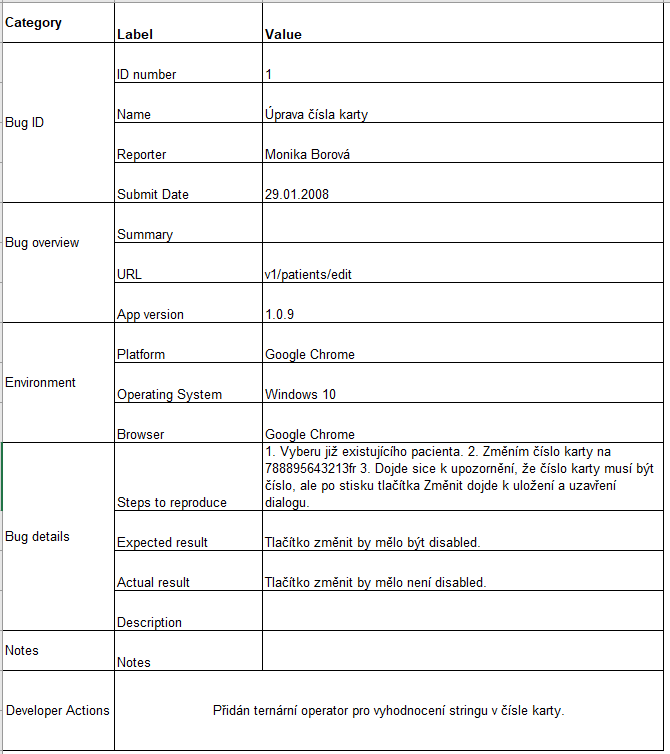
\includegraphics[width=15cm]{../bugReport.png}
	\caption{Oznámení chyby.}
	\label{fig:bugReport}
\end{figure}

\myparagraph{Nasazení}

Server pro nasazení testovacího prostředí byl poskytnut autorem. Jelikož jde o~Windows Server 2012, proběhlo vypublikování do internetu s~pomocí Internet Information Services (dále jen IIS), což je služba pro obsluhu příchozích požadavků na server. Výpis aplikací v~IIS je zobrazen na obrázku \ref{fig:applicationPools}. Aplikační pool \textit{SesterskaAplikace} je pool, který na dotázání vrací HTML soubor, který spouští celý frontend aplikace. Aplikační pool \textit{UrgentAppApi} je pool pod kterým běží server, který~naslouchá požadavky na dotyčném portu. Je nutné daným aplikačním poolům nastavit cestu, kde mají dotyčné soubory nutné pro chod aplikace hledat. Kořenová cesta je defaultně \textit{C:\textbackslash inetpub\textbackslash wwwroot}, kde je obsažena složka se jménem daného poolu. Také je potřeba nastavit adresu či IP adresu s~portem\footnote{Daný port je potřeba také otevřít ve Windows Firewallu jako inbound rule.}.  


\begin{figure} [H]
	\includegraphics[width=15cm]{../applicationPools.png}
	\caption{Aplikační pooly IIS.}
	\label{fig:applicationPools}
\end{figure}

\subsection{Nástroje}
\label{sec:nastroje}

\begin{itemize}
	\item Visual Studio 2015 \\
	Integrované vývojové prostředí (Integrated Development Environment dále jen IDE), které bylo využito v~této práci pro vývoj backendu v~C\# od firmy Microsoft. 
	\item Visual Studio Code \\
	Open source IDE, které bylo využito v~této práci pro vývoj frontendové části v~HTML, CSS a~ReactJS.
	\item Node Packager Module \\
	Neboli NPM je správce a~registr balíčků (knihoven) . Jedná se o~online úložiště JavaScript knihoven, které si může kdokoliv stáhnout a~použít ve svých projektech. Jedná se také o~verzovací nástroj, který hlídá závislosti a~podporované verze mezi danými závislostmi. 
	\item Nugget \\
	Nugget je podobně jako NPM nástroj, který je dodáván jako rozšíření pro Visual Studio IDE. Slouží také jako online úložiště knihoven a~registr, který hlídá závislosti mezi danými knihovnami. Je určen výhradně pro vývojové prostředí aplikací firmy Microsoft.
	\item Postman \\
	Postman je aplikace firmy Google, která funguje s~HTTP API rozhraními. Jde o~aplikaci, která snadno sestavuje požadavky a~čitelně prezentuje odpovědi ze serveru.
	\item Umlet \\
	Freeware aplikace pomocí které lze vytvářet jednoduché UML diagramy. Nicméně byla nedostačující co se týče uživatelského pohodlí a~nabízených grafických komponent.
	\item Draw.io \\
	Bohatý freeware nástroj pro vytváření všech typů UML diagramů. Obsahuje také nepřeberné množství hotových grafických komponent (firewall, databázový server atd.) a~obsahuje velké množství modifikací. Existuje jako webová i~stand-alone aplikace.
\end{itemize}

\section{Závěr}

Cílem této práce bylo vytvořit aplikaci pro personál urgentního příjmu Fakultní nemocnice Ostrava, pomocí které by bylo možné ovládat RTLS na uživatelské úrovni. Cílem bylo tedy v~první řadě seznámit se s~nynější situací na urgentním příjmu. Pochopit a~lokalizovat problémy, které trápily toto oddělení. Poté bylo potřeba tyto poznátky přenést do užitkových a~vývojových diagramů. Na základě těchto komplexních diagramů dále představit návrhy uživatelského prostředí aplikace a~paralelně přitom sestavovat backendovou část pro chod aplikace. Po schválení všemi zúčastněnými lidmi zbývalo naprogramovat podle návrhu skutečnou frontendovou část. V~průběhu vývoje aktivně probíhala komunikace s~koncovými uživateli produktu, kterými jsou personál urgentního příjmu Fakultní nemocnice Ostrava. Aktivně se komunikovalo z důvodu zlepšení, problémů či funkcionality. Po důkladném testování bylo řešení nasazeno v~produkčním prostředí, kde poté proběhlo testování v~reálném provozu. 

Práci na tomto projektu, kde byla zahrnuta široká škála dovedností lidí, byla velice obohacující. Bylo mi umožněno navrhnout řešení od úplného začátku (green field software development), přičemž toto řešení je poté používáno v~oblasti, kde je důraz na maximální nechybovost. Tato práce obsahuje počáteční analýzu, návrh uživatelského rozhraní, vývoj obou částí aplikace, testování a~nakonec nasazení. Budoucí motivací je dále statistické zpracování výsledků a~určení rizikových míst (bottleneck), kde dochází ke zbrždění vyšetřovacího cyklu pacienta. Tento statistický výstup poté povede k~analýze a~zlepšení těchto nedostatků, které zefektivní celé oddělení a~tím i~zvýší kvalitu vyšetření. 

První kapitola ze čtyř pojednává o~úvodu, motivaci a~cílech této diplomové práce. Pro praktickou část bylo potřeba zanalyzovat dostupné technologie pro tvorbu webových aplikací, čemuž se věnuje kapitola 2, kde je i~mimojiné probrána architektura řešení, klady a~zápory technologií a~způsob komunikace mezi frontendem a~backendem. Předposlední kapitola pak pojednává o~vlastním návrhu řešení. V~této části práce byla popsána analýza situace před dodáním softwaru, postup vývoje a~detailní vysvětlení architektury aplikace. Poslední kapitola pak zhodnocuje celou práci a~nastiňuje budoucí motivaci, která pak uzavírá tuto diplomovou práci.
